\documentclass[12pt,a4paper]{report}
\usepackage[utf8]{inputenc}
\usepackage[english]{babel}
\usepackage{graphicx}
\usepackage{pgfplots}
\usepackage[left=2cm,right=2cm,top=2cm,bottom=2cm]{geometry}

\graphicspath{{../../out/}}

\pgfplotsset{
	compat=1.17,
	no markers
}

\author{Andrei N. Onea}
\title{37212-cwk2-S-Object\_detection\_k83954ao}

\begin{document}
\maketitle

\subsection*{Experiment}

This assignment attempts to match an object from a reference image, in several benchmark images. The subject is the person Bernie Sanders, and the benchmark images provided represent different variations in rotation, scale, illumination, blurring etc. to test the performance of the object detector. The implementation has three parts. Part 1 deals with feature detection using own implementation of the Harris corner detector, Part 2 deals with feature description, and descriptors are constructed using the OpenCV built-in ORB framework, and finally Part 3 deals with feature matching, using own implementation of sum of squared differences with ratio test for discarding ambiguous matches. We will compare some results and provide our thoughts on the experiment.

\subsection*{Part 1: Feature detection}

The main steps for feature detection are: blur the gray-scaled image, compute the image derivatives using Sobel operators, compute the combinations of the image derivatives, apply a Gaussian blur on the combinations, compute the matrix, compute the cornerness function $R=det(M) - \alpha \times trace(M)^{2}$ for each pixel and finally filter the corners using own implementation for non-maxima suppression with thresholding. Keypoints are then created from the filtered values. In Figure \ref{fig:kp} we see the evolution of the number of keypoints as the threshold value changes. We notice an exponential decrease, as there are many fluctuations in the values at smaller scale, but as the values increase, they are increasingly more the same, so the constant lines at the end appear.

Our choice of threshold is 80. We chose the value empirically, as we tried to minimize the number of features detected outside of Bernie's shape. The Appendix contains all the keypoints detected in all images. Discussion on the performance of the feature detection implementation will be made in Part 3.

\begin{figure}[ht]
	\centering
	\begin{tikzpicture}
	\begin{semilogyaxis}[
		title={Number of keypoints over threshold value},
		xlabel={Threshold},
		ylabel={Keypoints}
	]
	\addplot[black] table {../../out/plot.txt};
	\end{semilogyaxis}
	\end{tikzpicture}
	\caption{Variation in the number of keypoints as the threshold value increases}
	\label{fig:kp}
\end{figure}

\subsection*{Part 2: Feature description}

For this step, we used the built-in ORB framework in the OpenCV package. Figure \ref{fig:com} has side-by-side the keypoints detected by our implementation with the keypoints detected by ORB. We can see that in this regard, the performance of your feature detector is almost indistinguishable from the ORB detector.

\begin{figure}[ht]
	\centering
	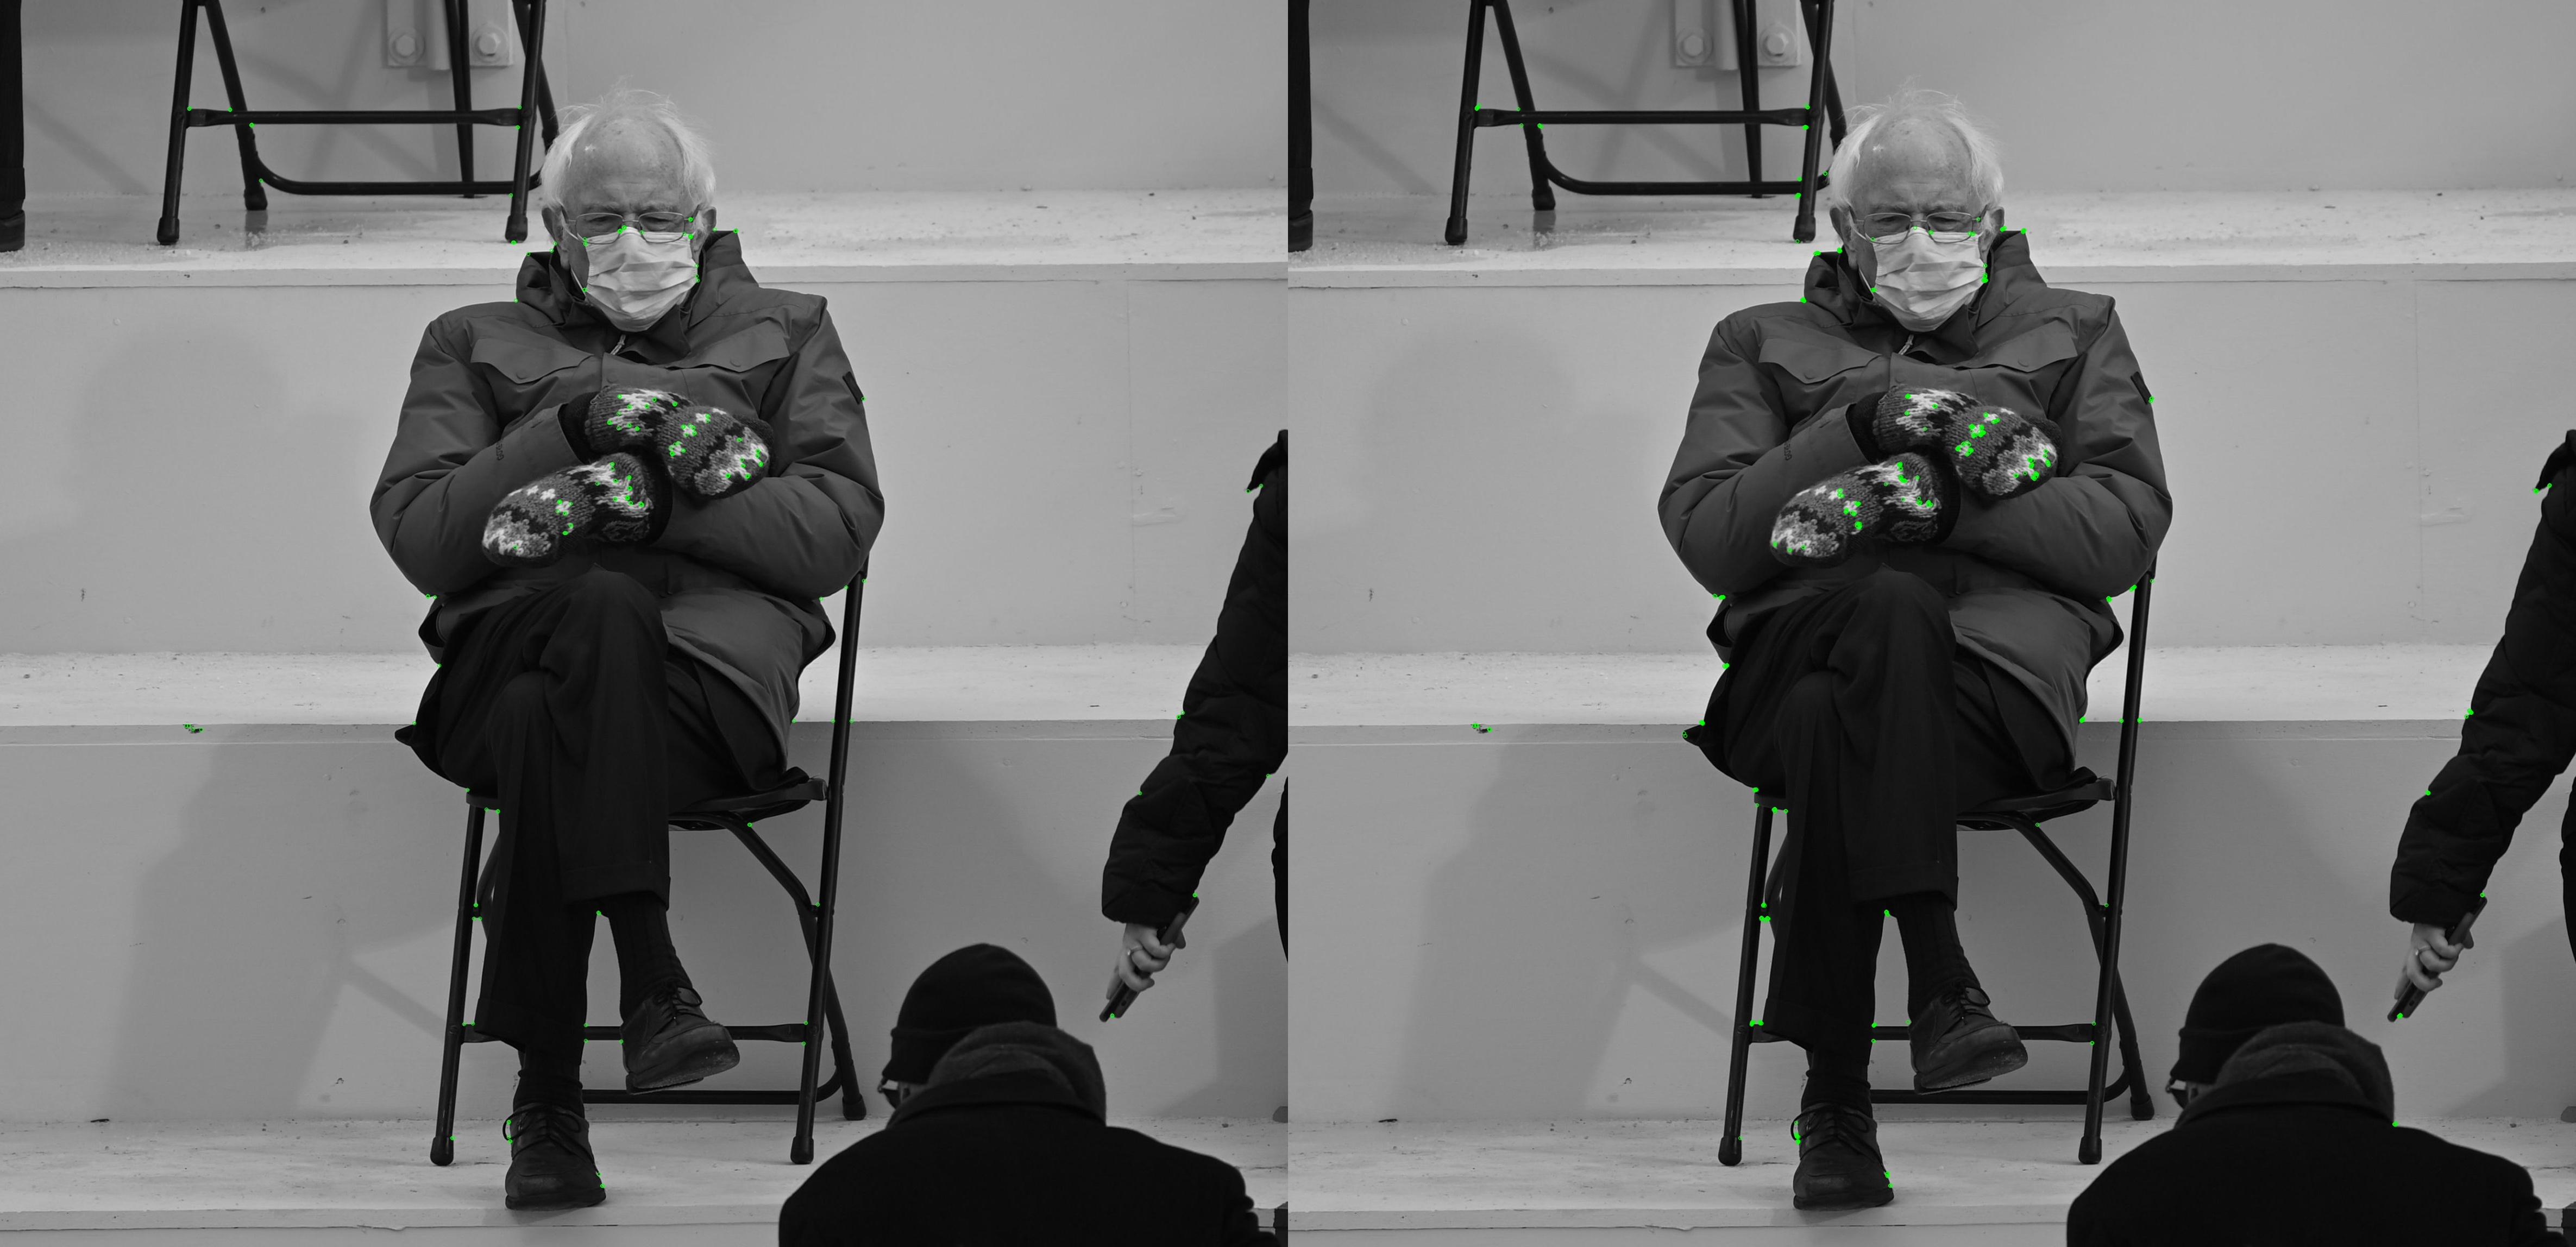
\includegraphics[width=\textwidth]{comparison}
	\caption{(left) our implementation, (right) ORB detect function}
	\label{fig:com}
\end{figure}

\subsection*{Part 3: Feature matching}
The last step is to try matching the features from the reference image with features from the benchmark images. This is done by computing the sum of squared differences between two feature windows. This is done for every combination of features and then the smallest distance is picked. Because this might return ambiguous results, the second smallest distance is also picked then a ratio between the first and the second is made. If this ratio is close to 1, then the match is discarded. We chose 0.9 as the threshold value for the ratio test, and 200 as the threshold value for the maximum distance for which a match is selected.

\clearpage
\subsubsection*{Rotated image}

\begin{figure}[ht]
	\centering
	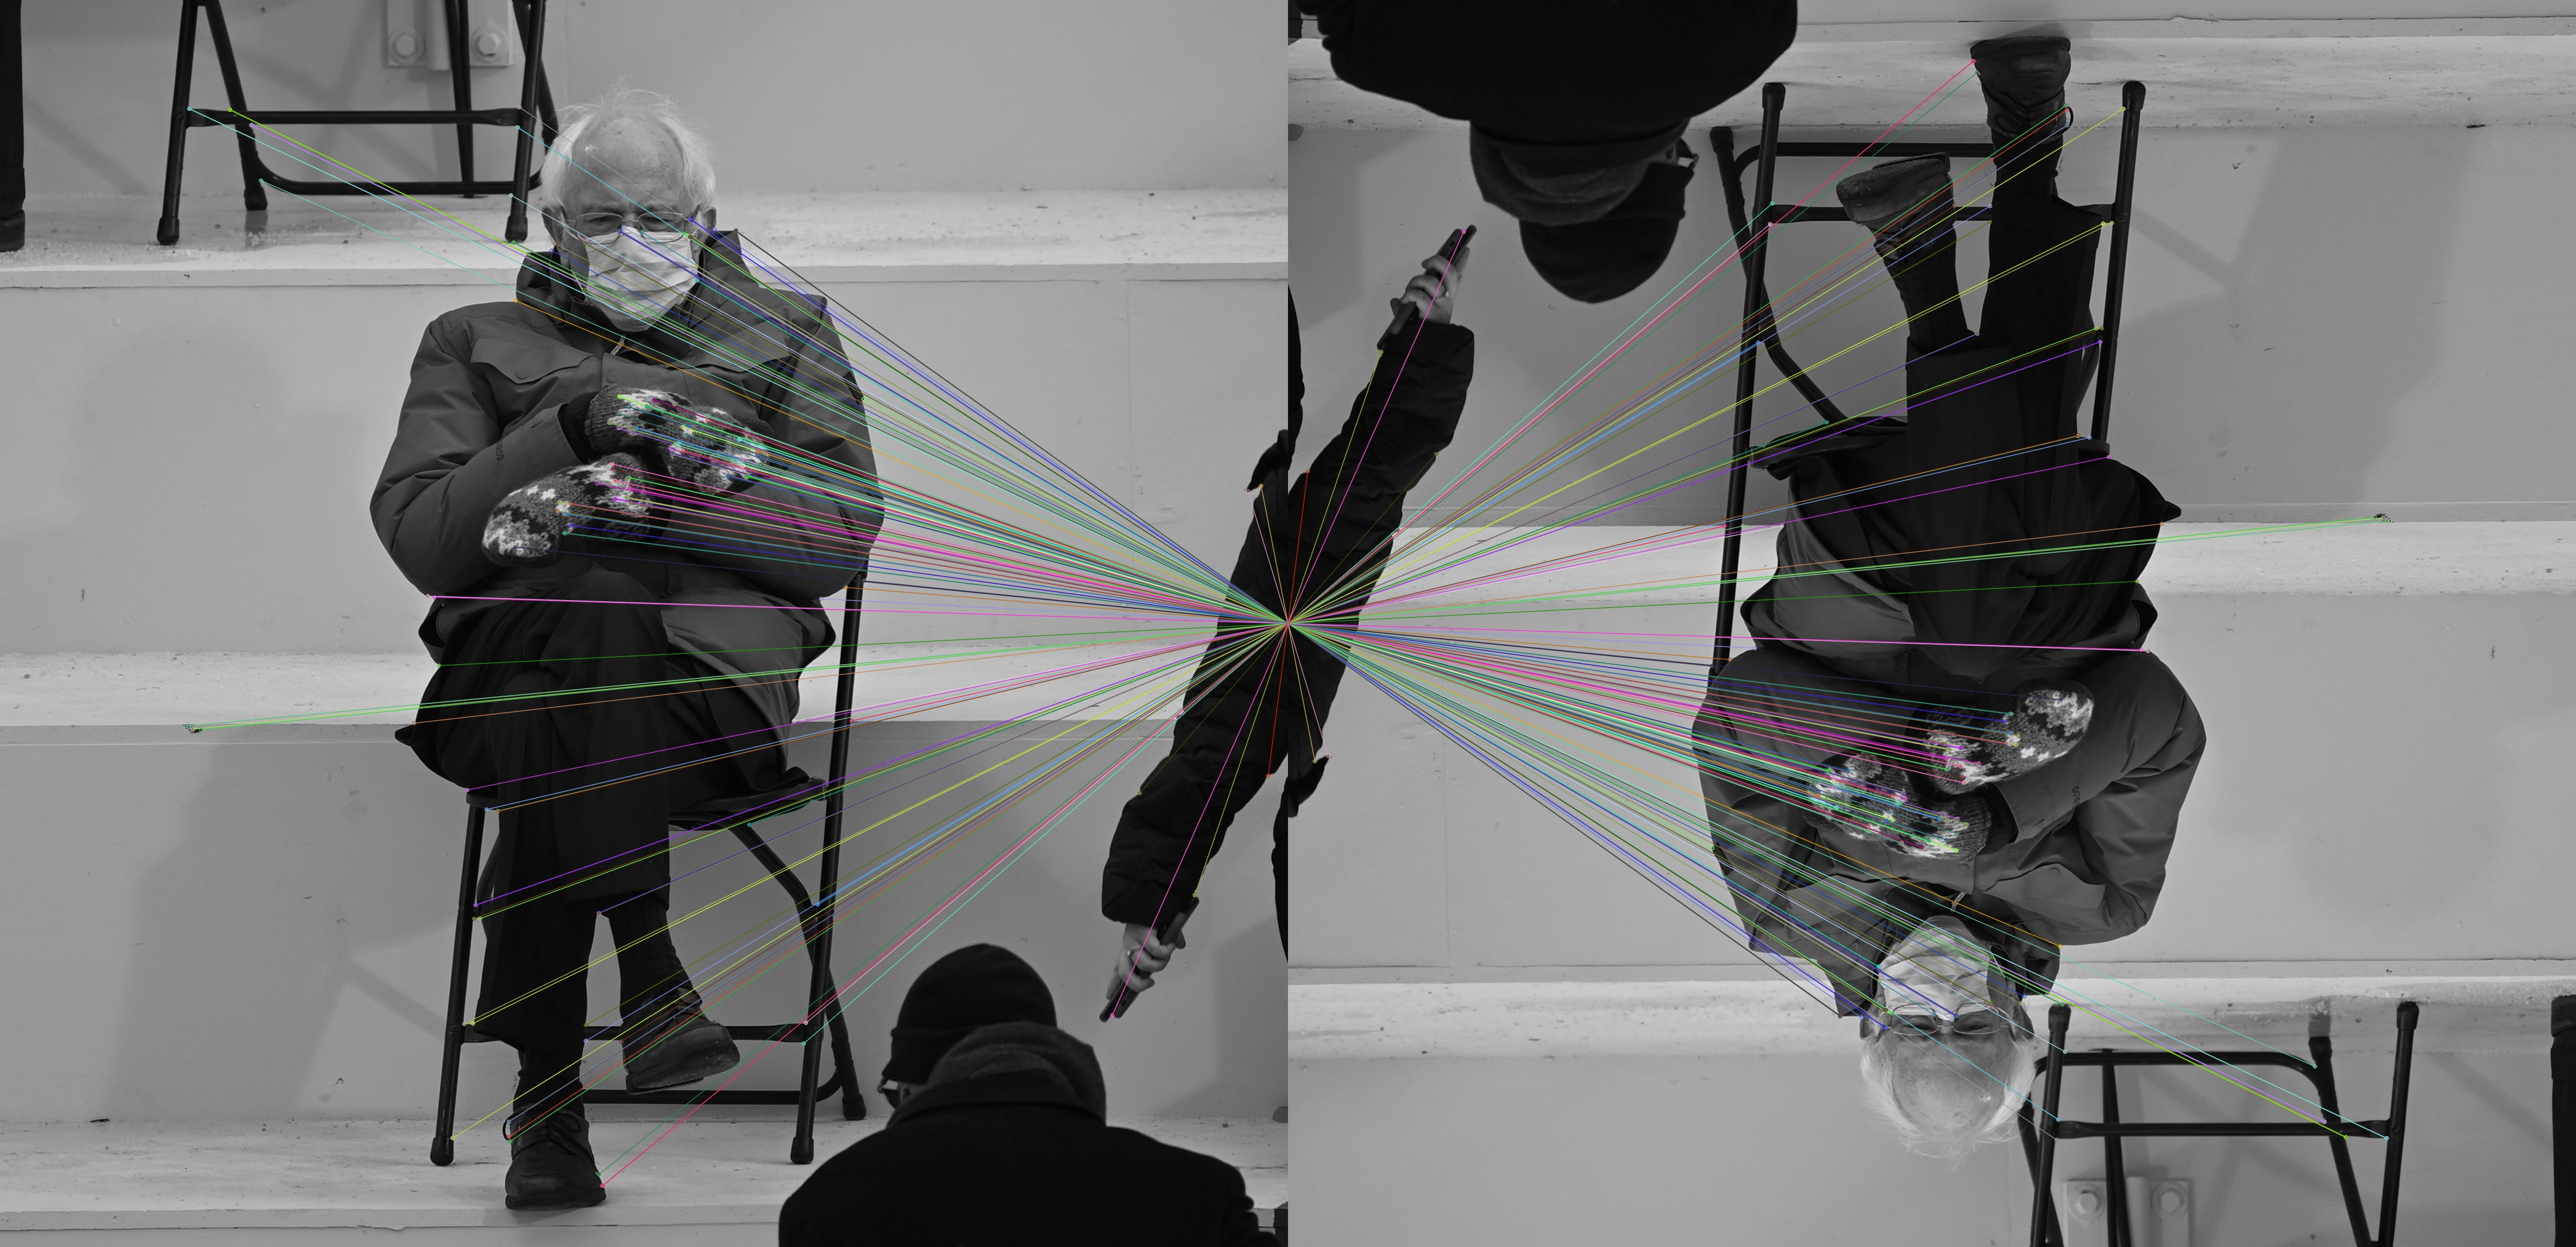
\includegraphics[width=\textwidth]{bernie180.jpg_match}
	\caption{Rotated image}
\end{figure}

Because the only variation is in rotation, the matcher gets all the features right.

\clearpage
\subsubsection*{Scaled image}

\begin{figure}[ht]
	\centering
	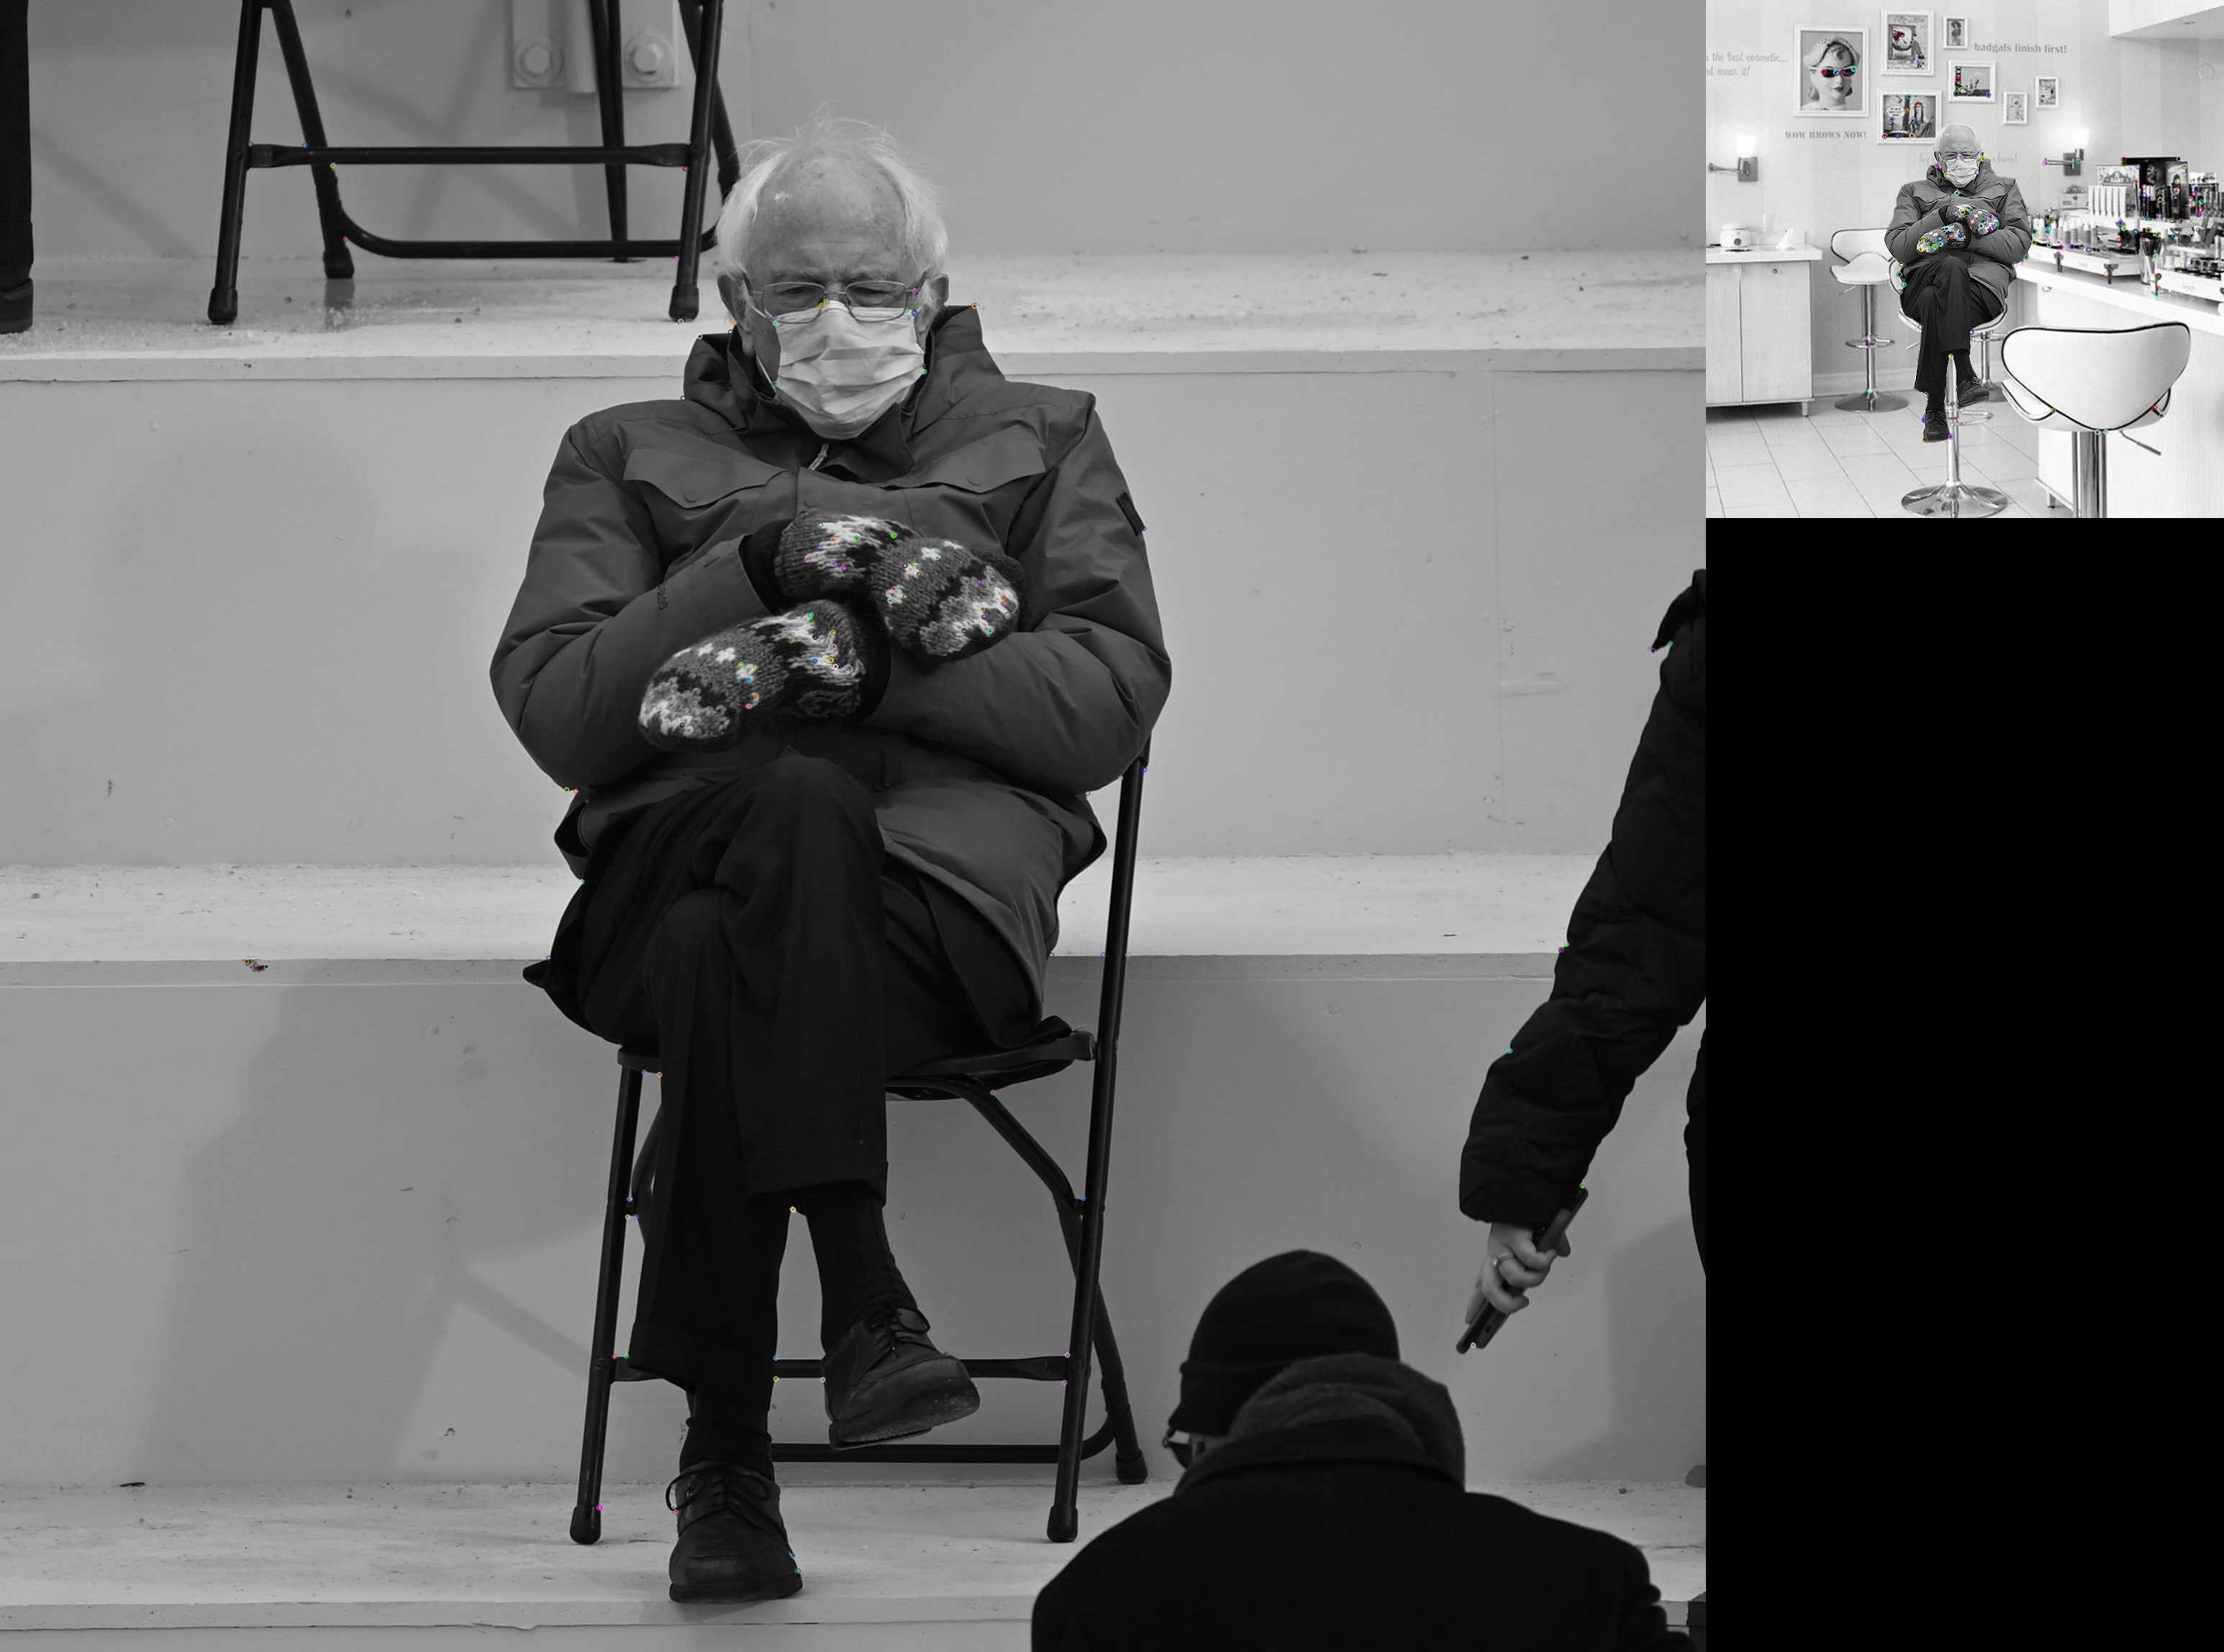
\includegraphics[width=\textwidth]{bernieBenefitBeautySalon.jpeg_match}
	\caption{Scaled image}
\end{figure}

As it will be the case with all scaled benchmark images, the matcher does not find any result. That is because our basic implementation is not scale invariant, meaning that it cannot detect changes in scale.

\clearpage
\subsubsection*{Blurred image}

\begin{figure}[ht]
	\centering
	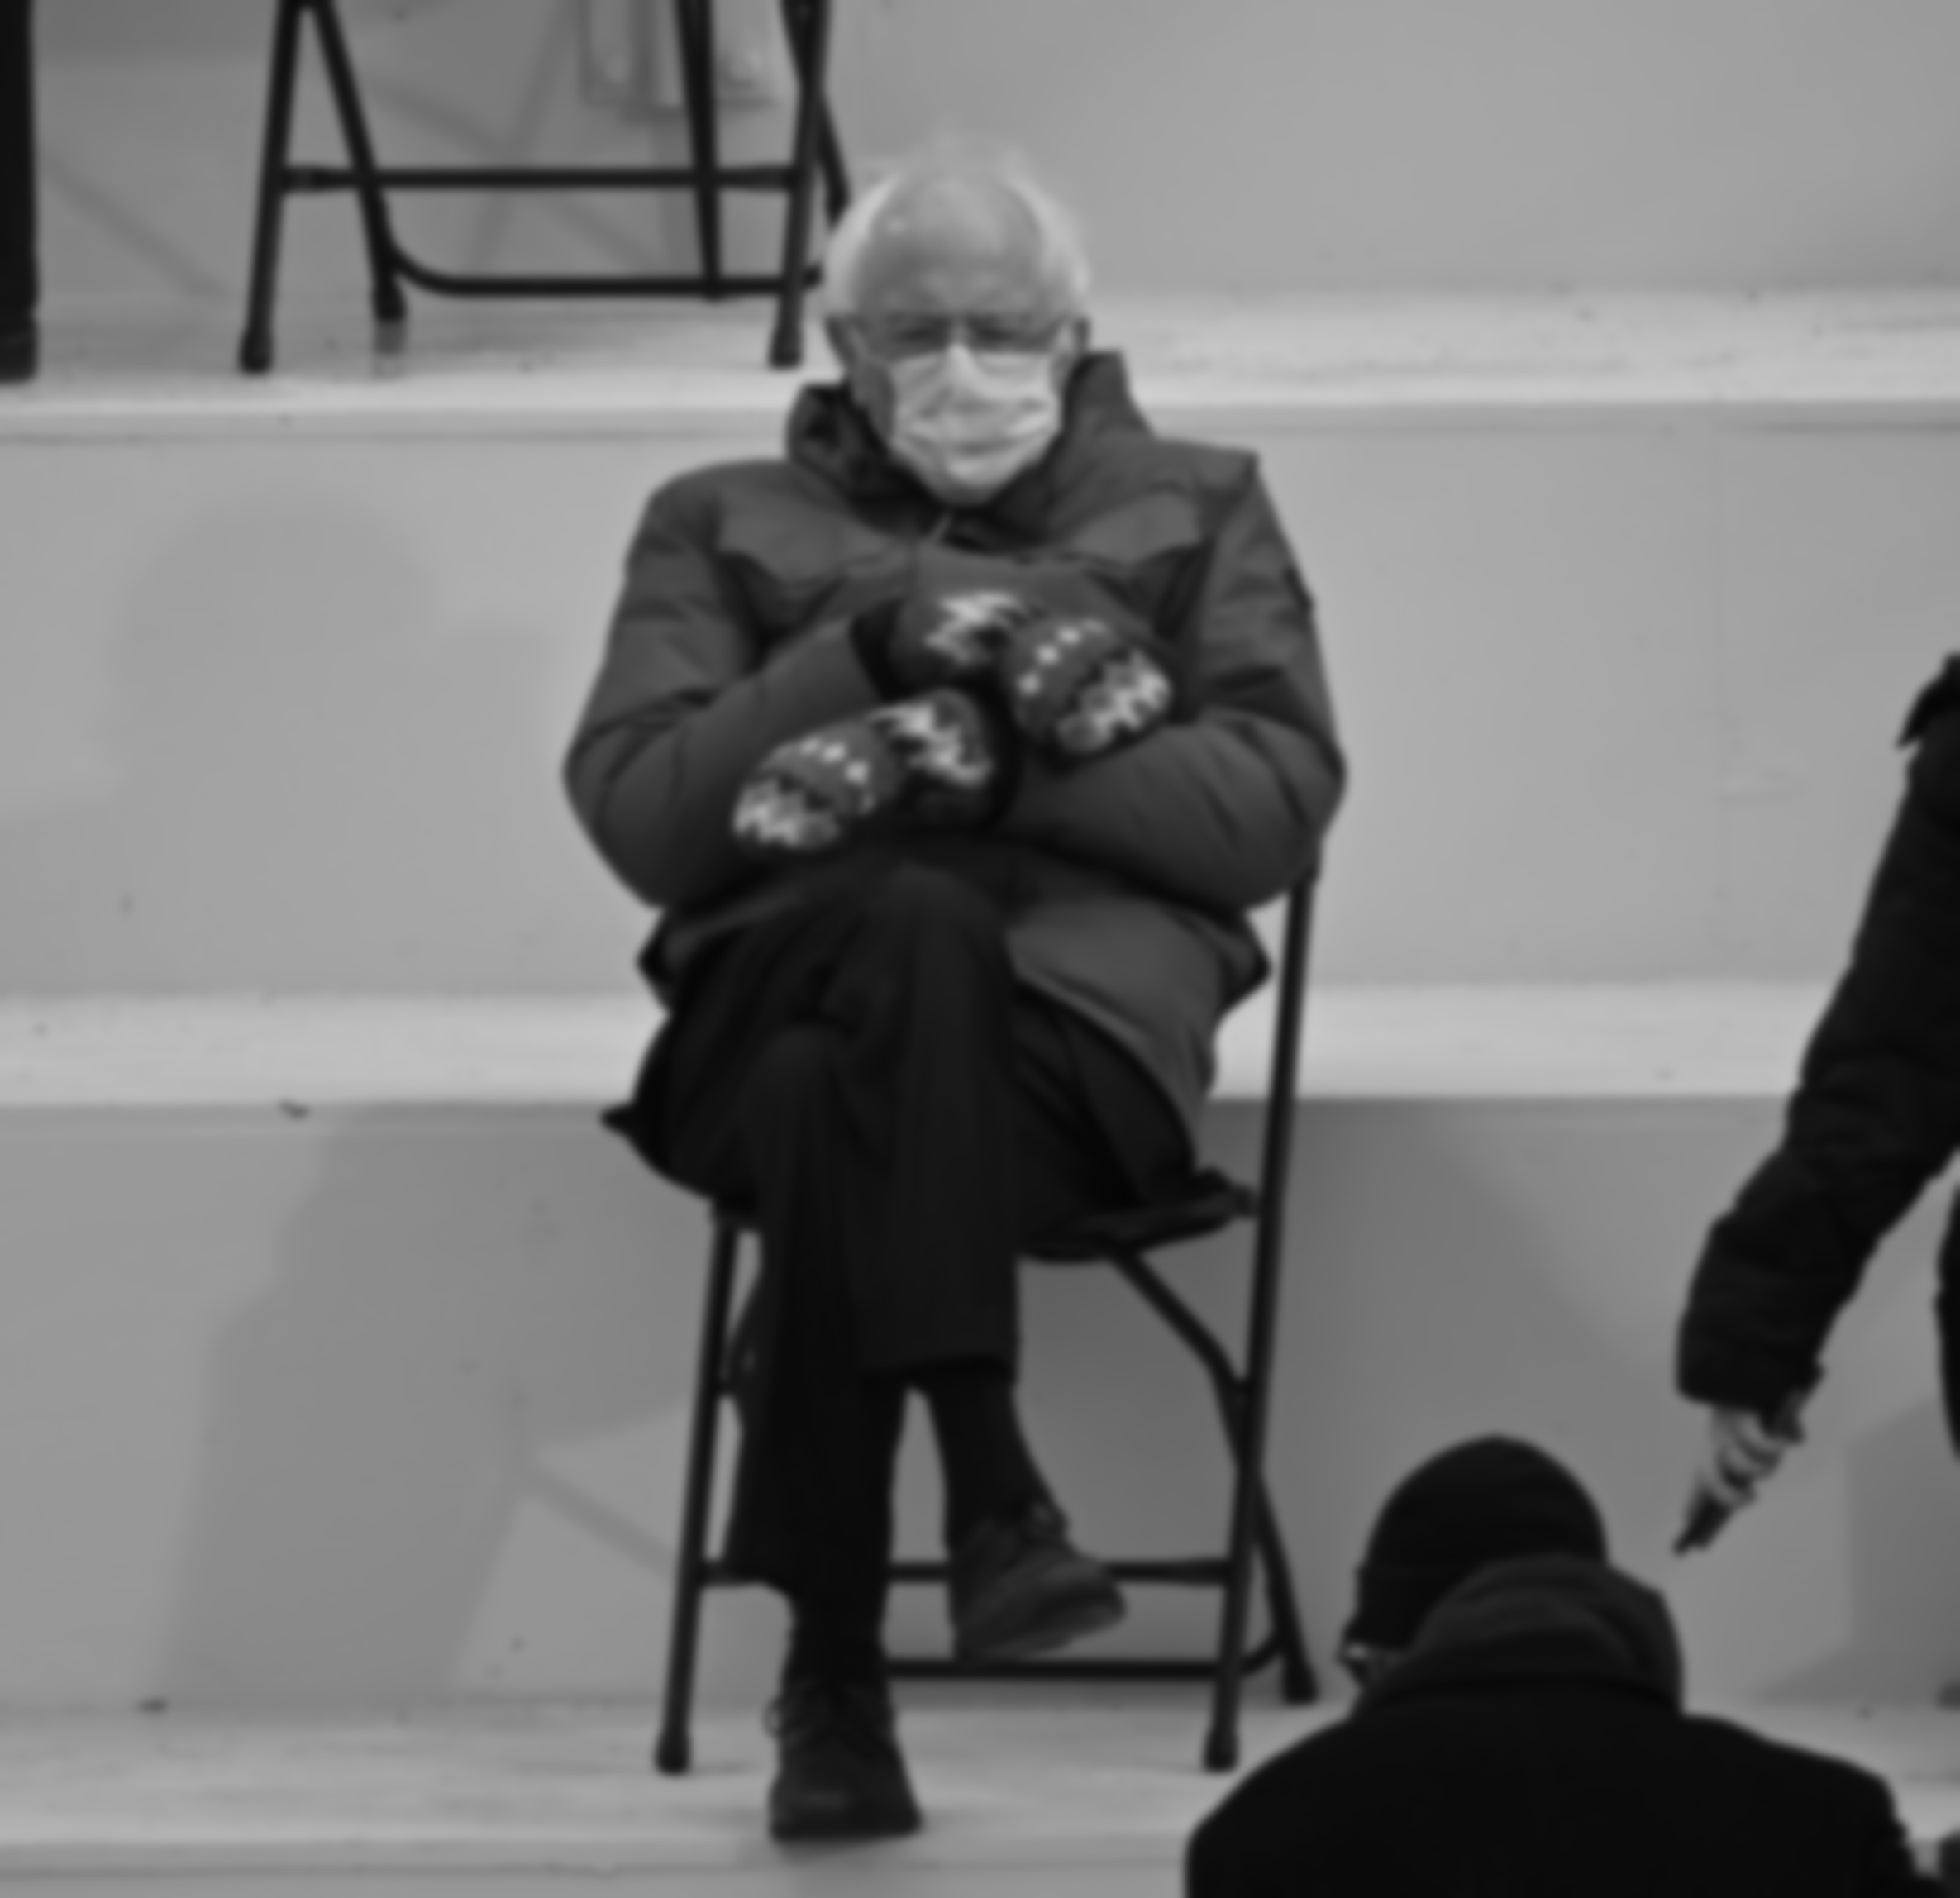
\includegraphics[width=\textwidth]{bernieMoreblurred.jpg_match}
	\caption{Blurred image}
\end{figure}

Because the image is already quite blurred, fine detail is lost and the detector takes any flat surface as a corner, and only distinguishes flat surfaces from edges. That is why there are so many keypoints. However, there is one single feature that is correctly matched, that is one point on the glove, here represented in yellow.

\clearpage
\subsubsection*{Noisy image}

\begin{figure}[ht]
	\centering
	\includegraphics[width=\textwidth]{bernieNoisy2.png_match}
	\caption{Noisy image}
\end{figure}

Because the image is noisy, pixels are misinterpreted. There is a match, again on the glove, represented in cyan.

\clearpage
\subsubsection*{Pixelated image}

\begin{figure}[ht]
	\centering
	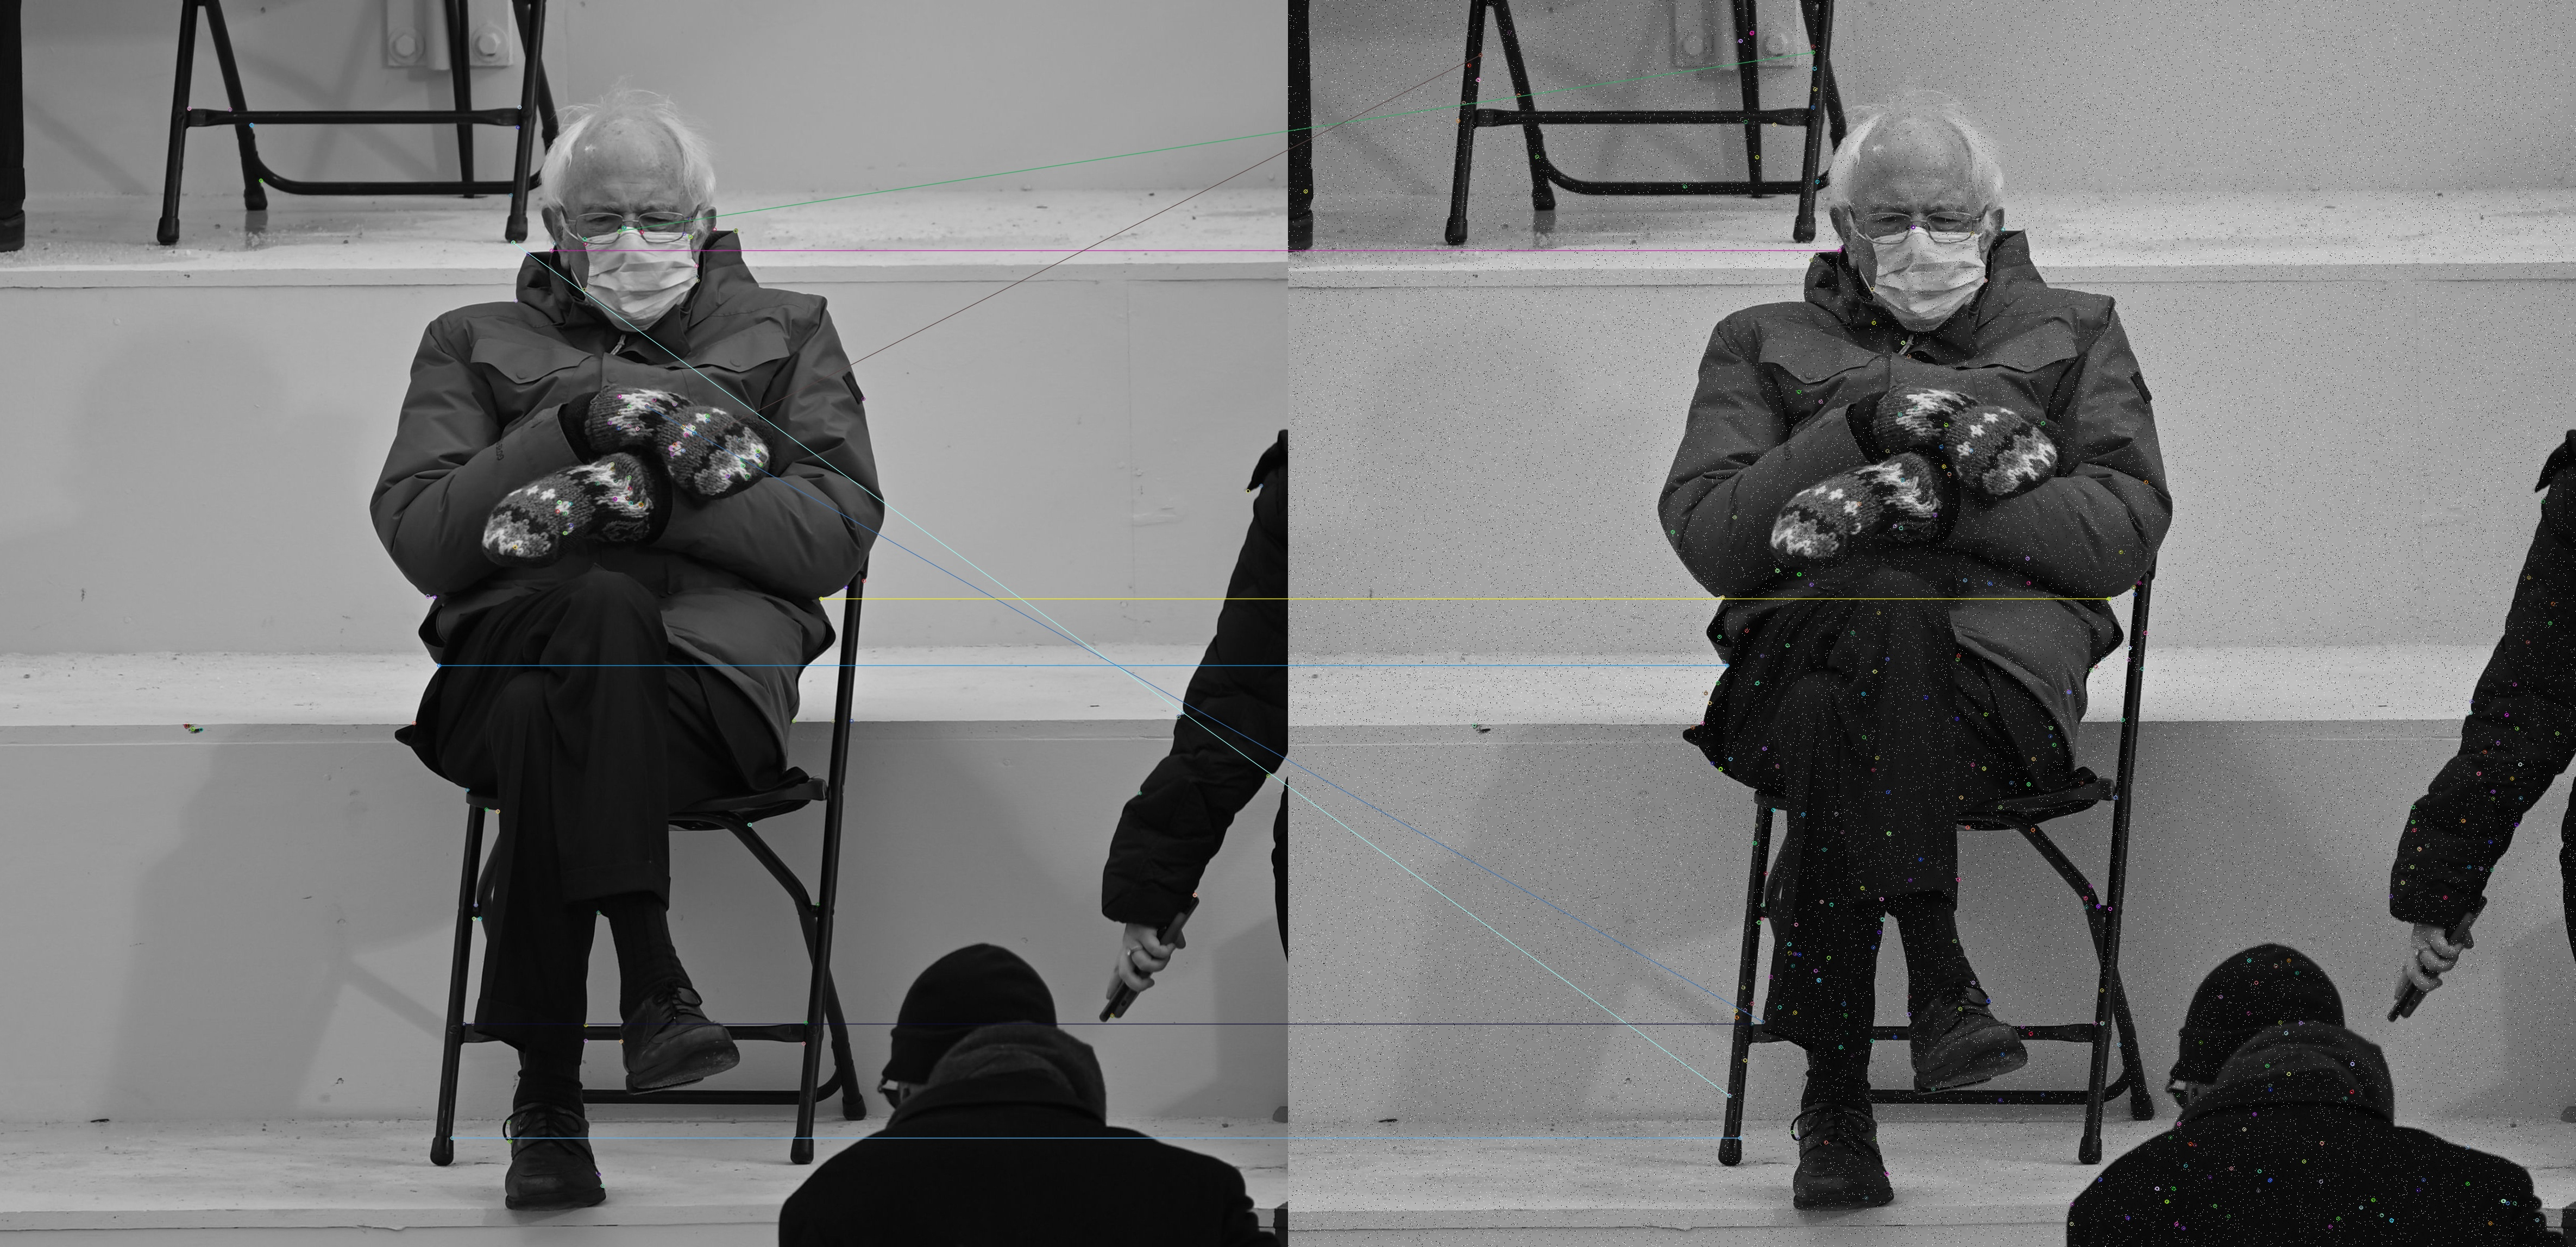
\includegraphics[width=\textwidth]{berniePixelated2.png_match}
	\caption{Pixelated image}
\end{figure}

This example is similar to the noisy image above, but the pixelated pattern is less impactful, thus more matches are correctly found.

\clearpage
\subsubsection*{Similar characters and scaled image}

\begin{figure}[ht]
	\centering
	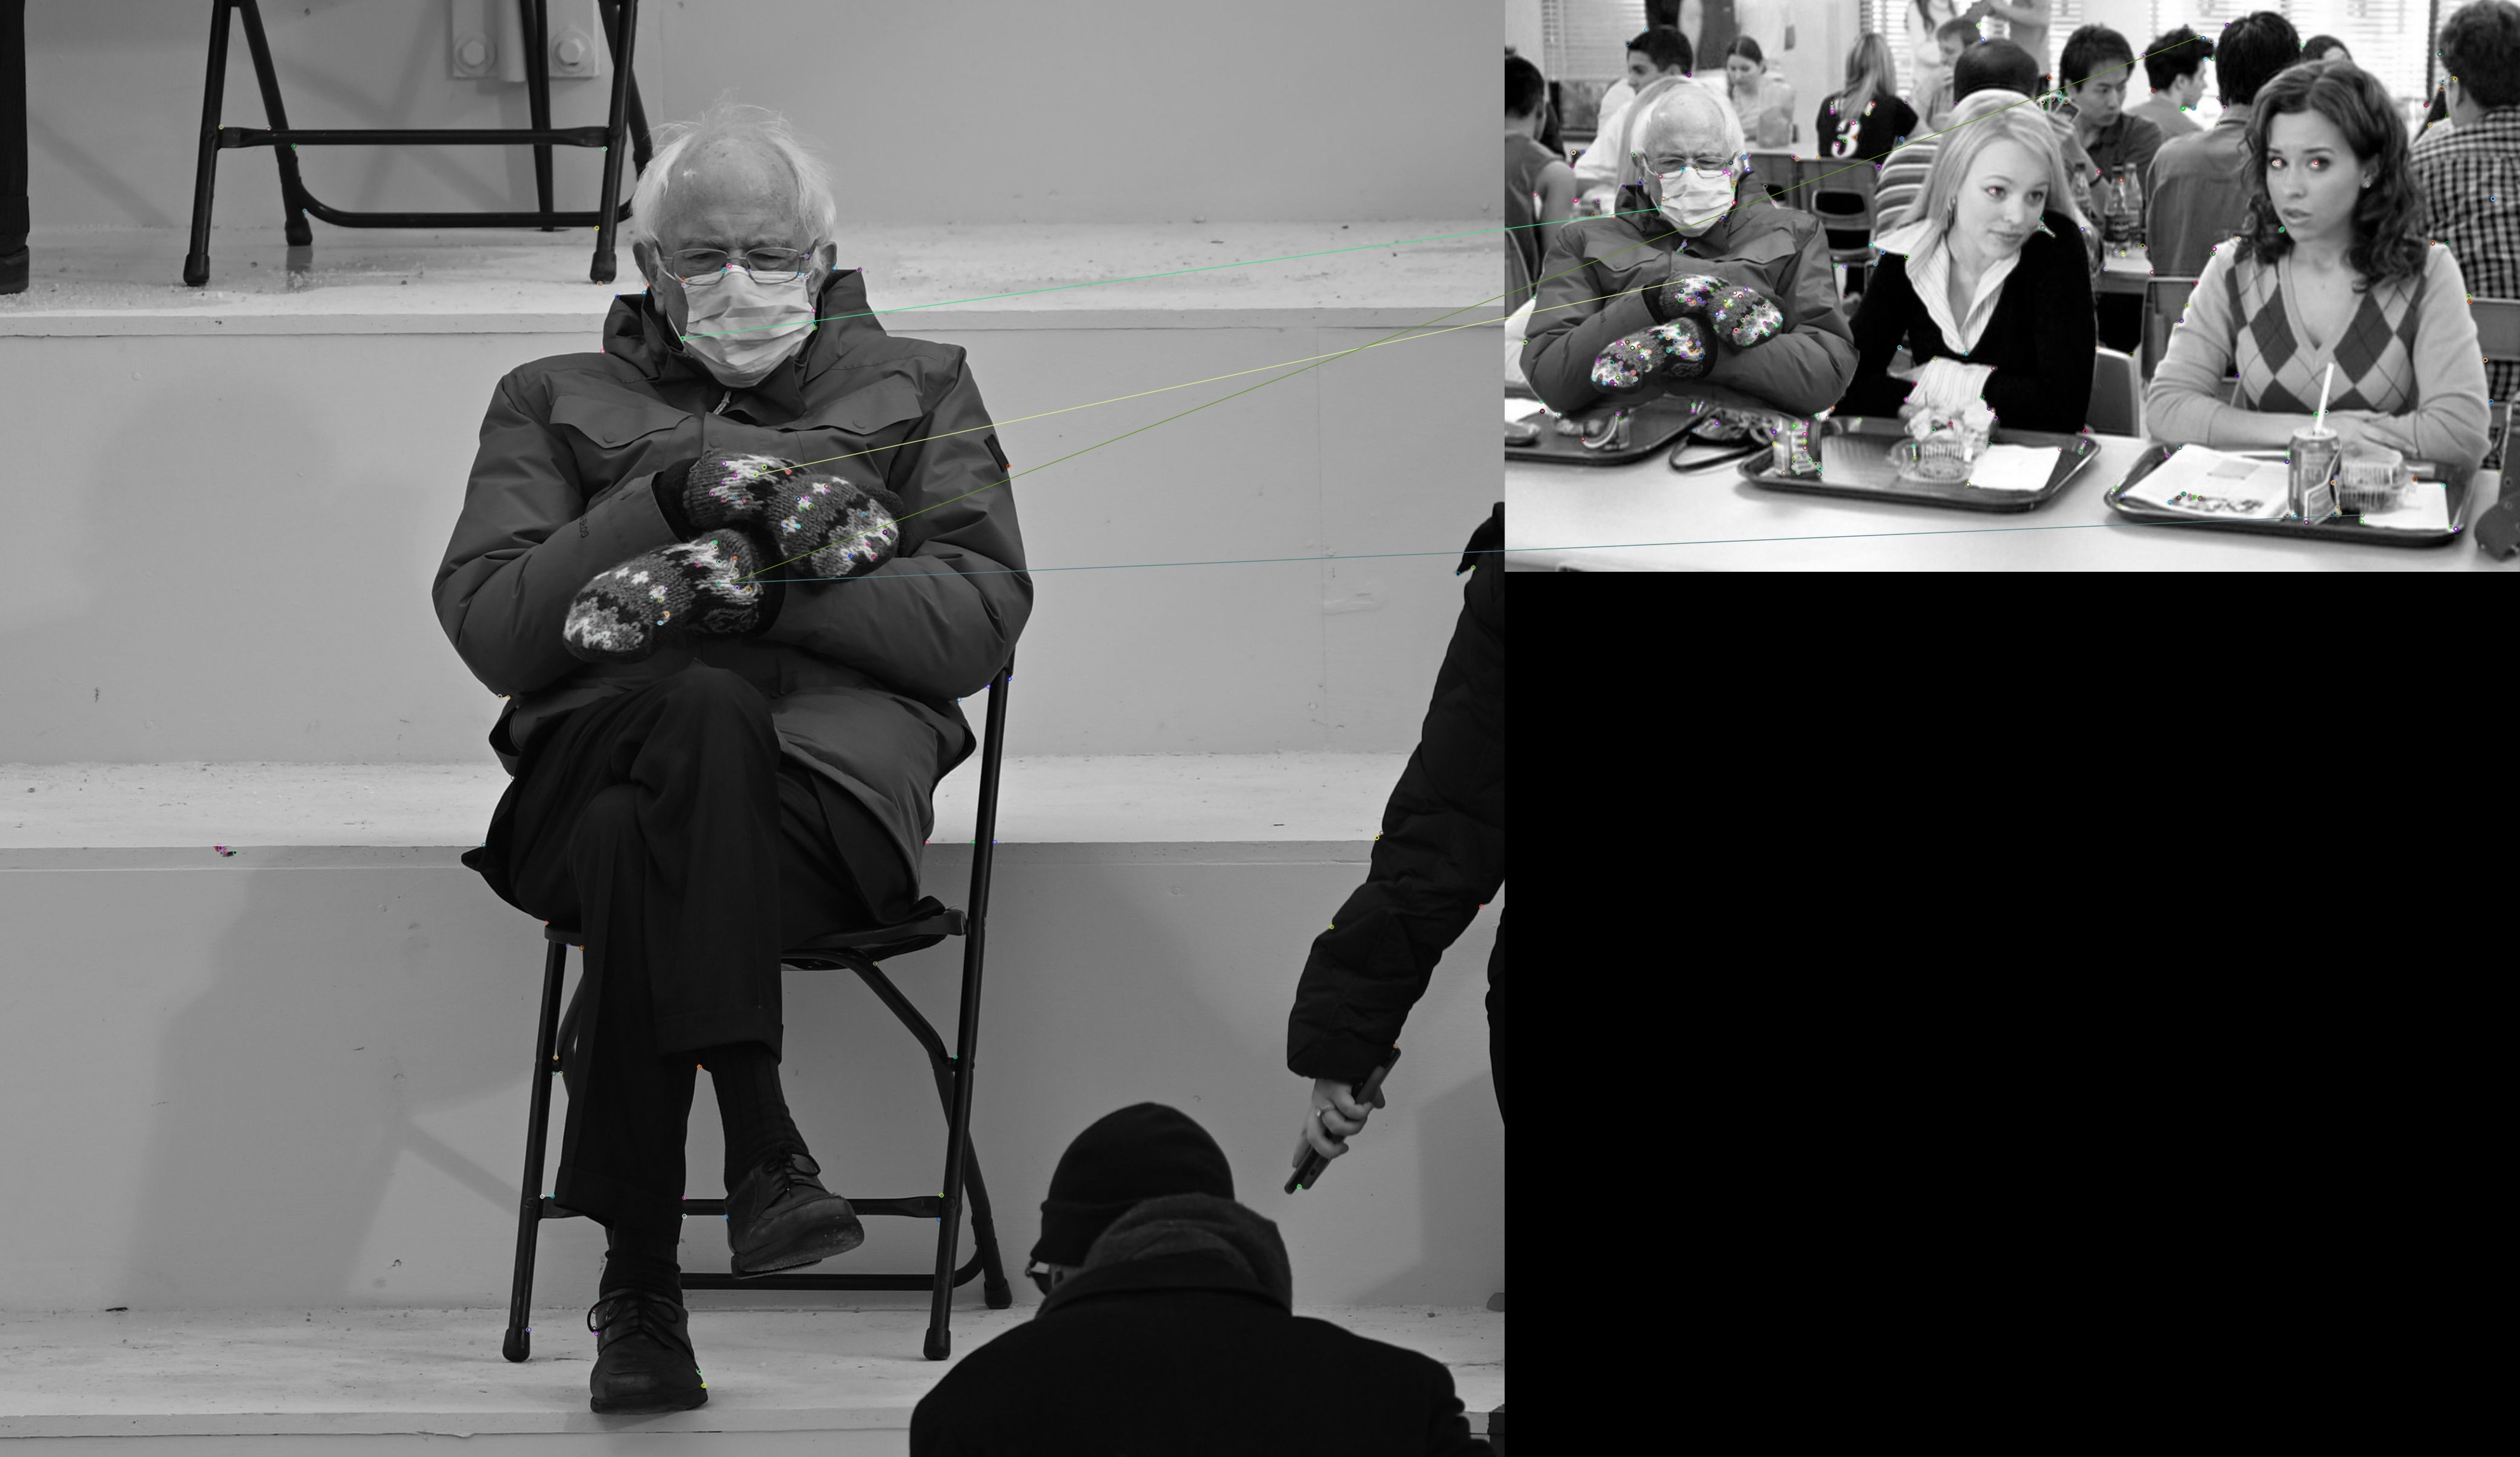
\includegraphics[width=\textwidth]{bernieShoolLunch.jpeg_match}
	\caption{Similar characters and scaled image}
\end{figure}

Surprisingly, there are two matches on the mask and the glove which correspond perfectly. The others are misinterpreted, as expected with images that have variations in scale.

\clearpage
\subsubsection*{Many characters and scaled image}

\begin{figure}[ht]
	\centering
	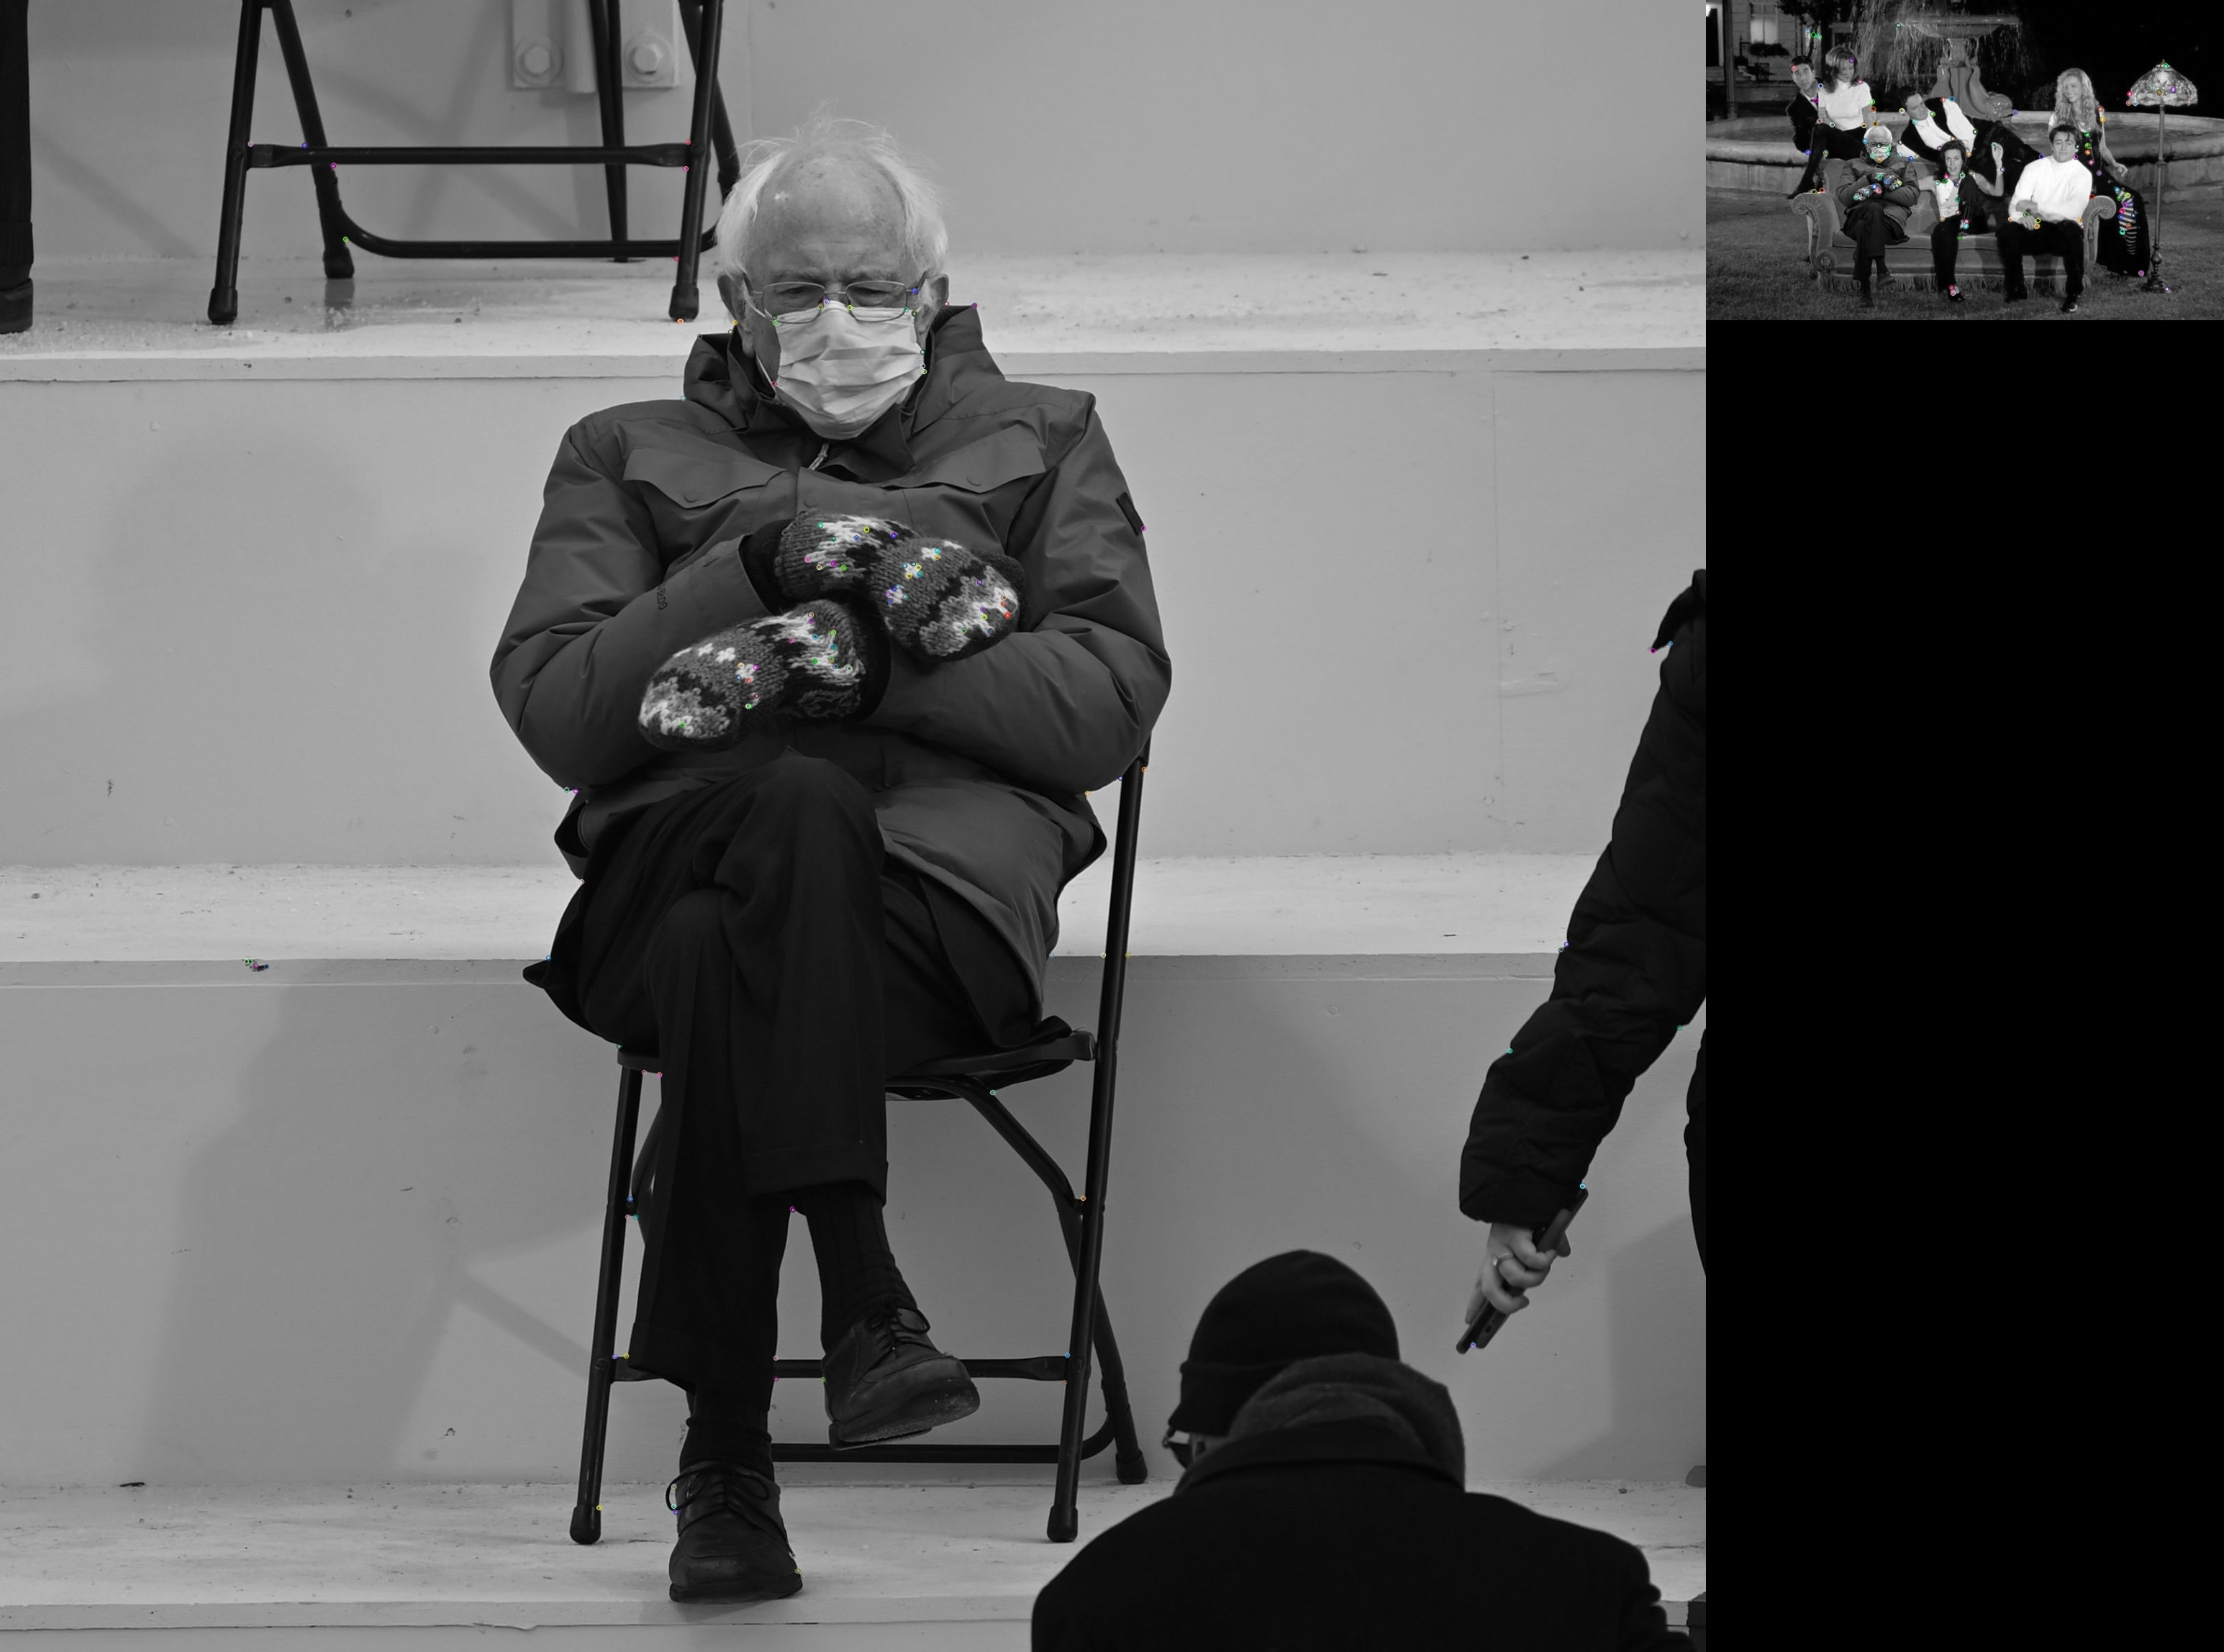
\includegraphics[width=\textwidth]{BernieFriends.png_match}
	\caption{Many characters and scaled image}
\end{figure}

A better example of why images with variations in scale do not produce good results. The distances are usually off in these cases and get discarded by the threshold test. Although features are present, no match is found.

\clearpage
\subsubsection*{Brighter image / Darker image}

\begin{figure}[ht]
	\centering
	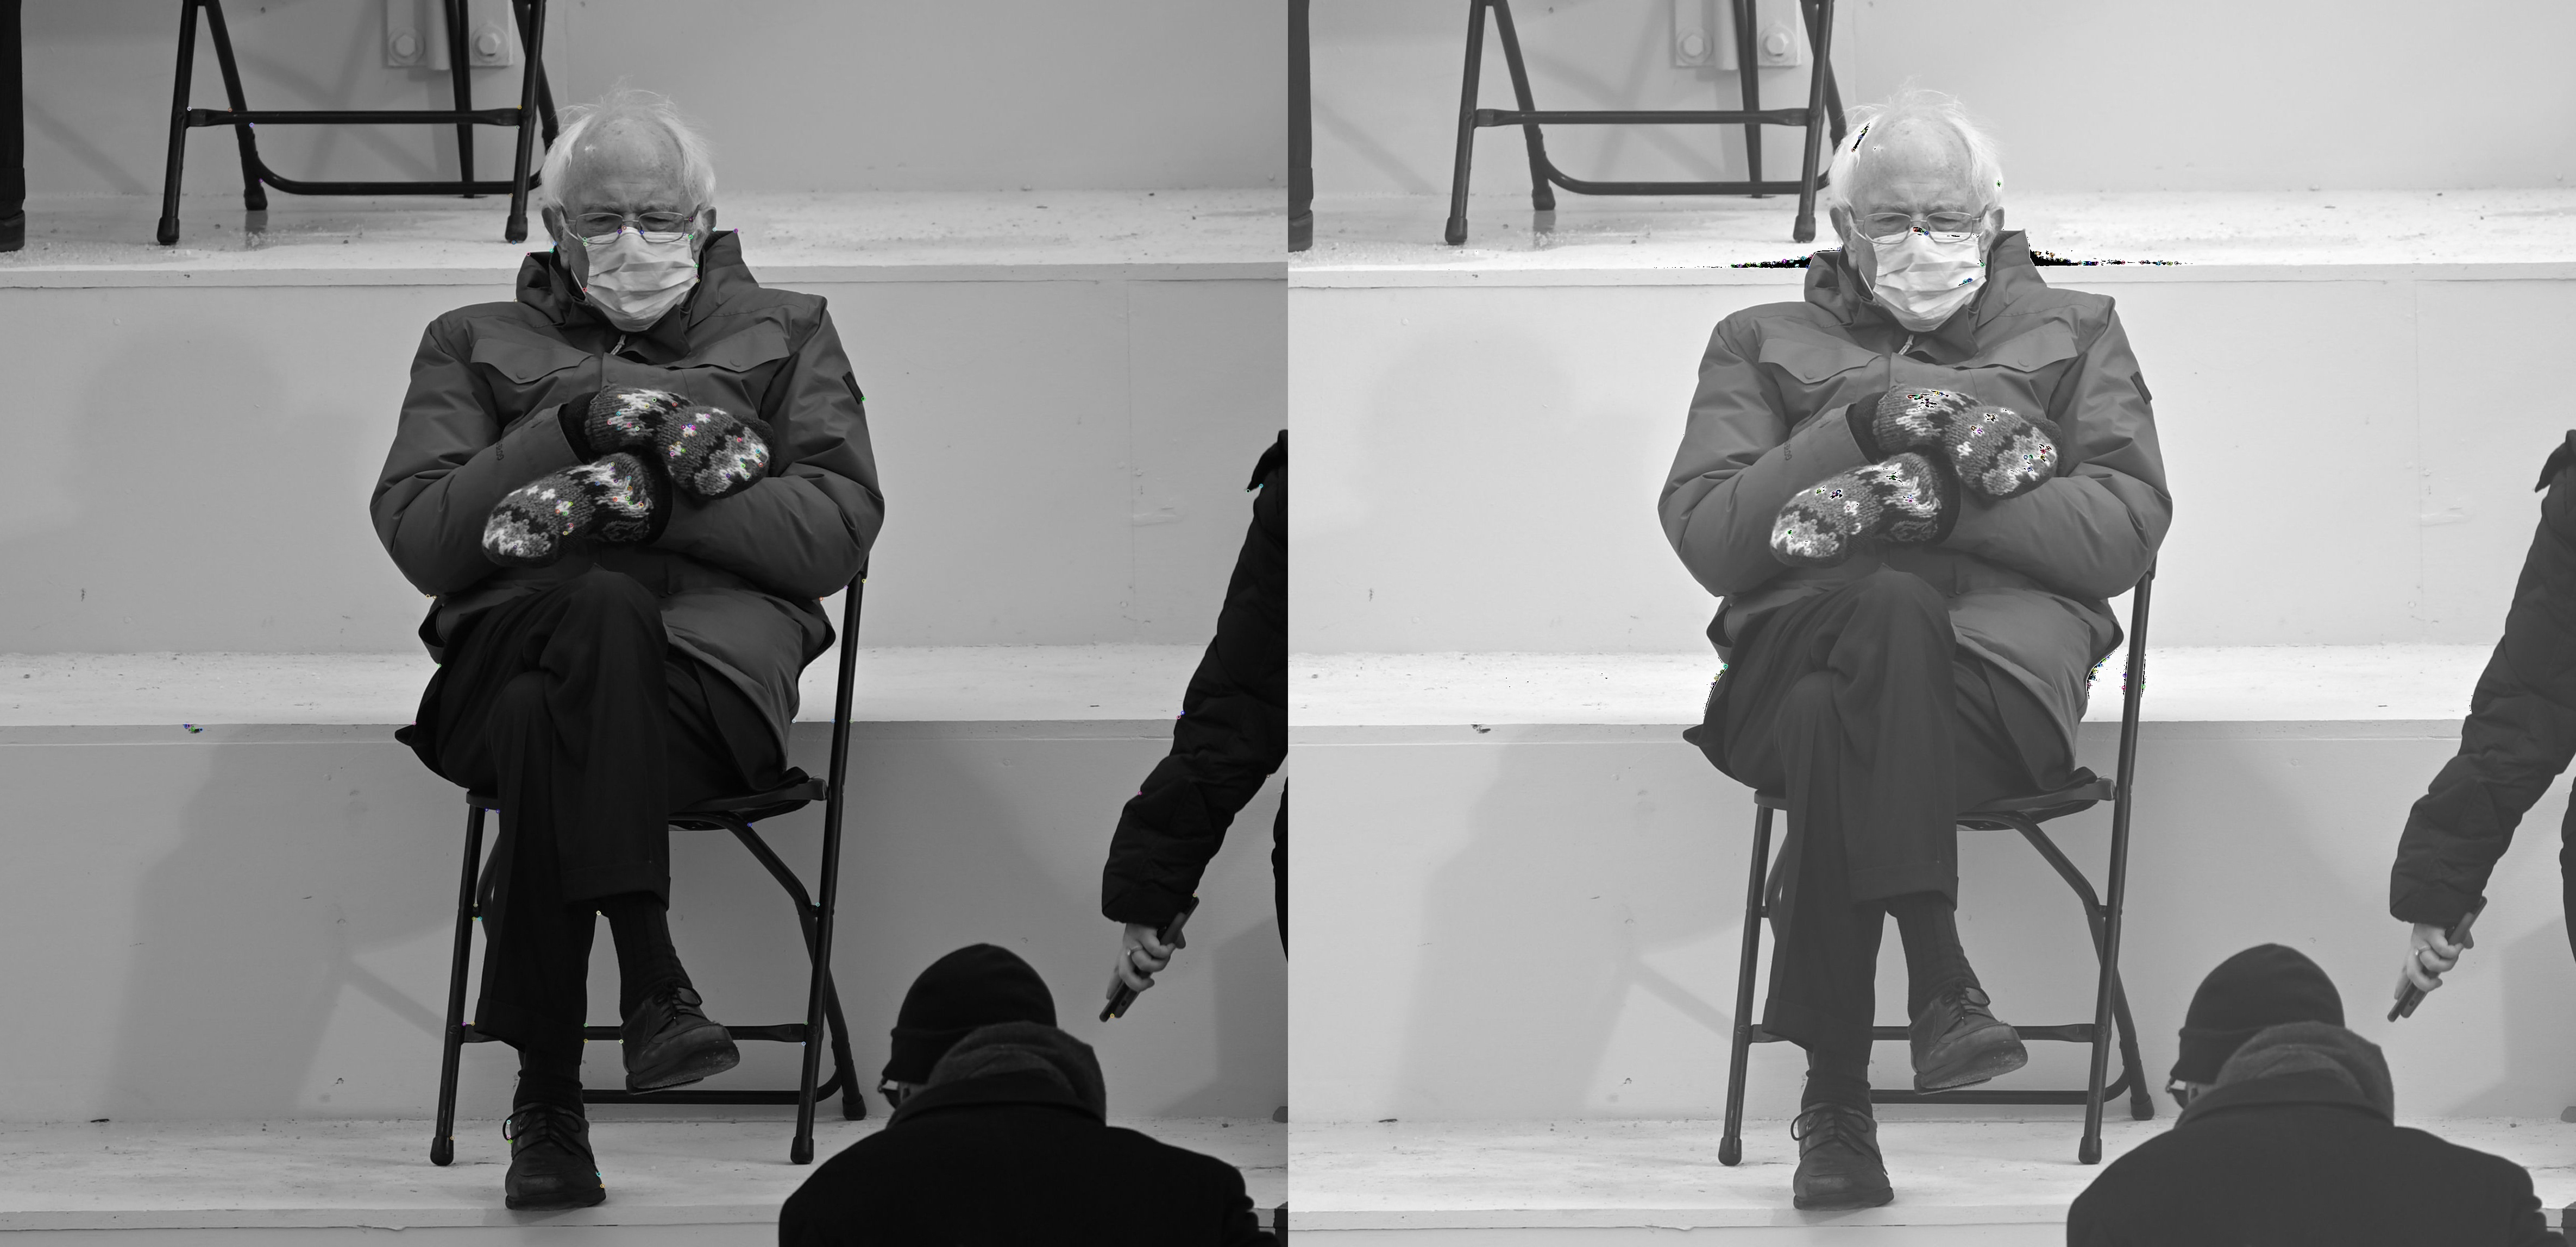
\includegraphics[width=\textwidth]{brighterBernie.jpg_match}
	\caption{Brighter image}
\end{figure}

\begin{figure}[ht]
	\centering
	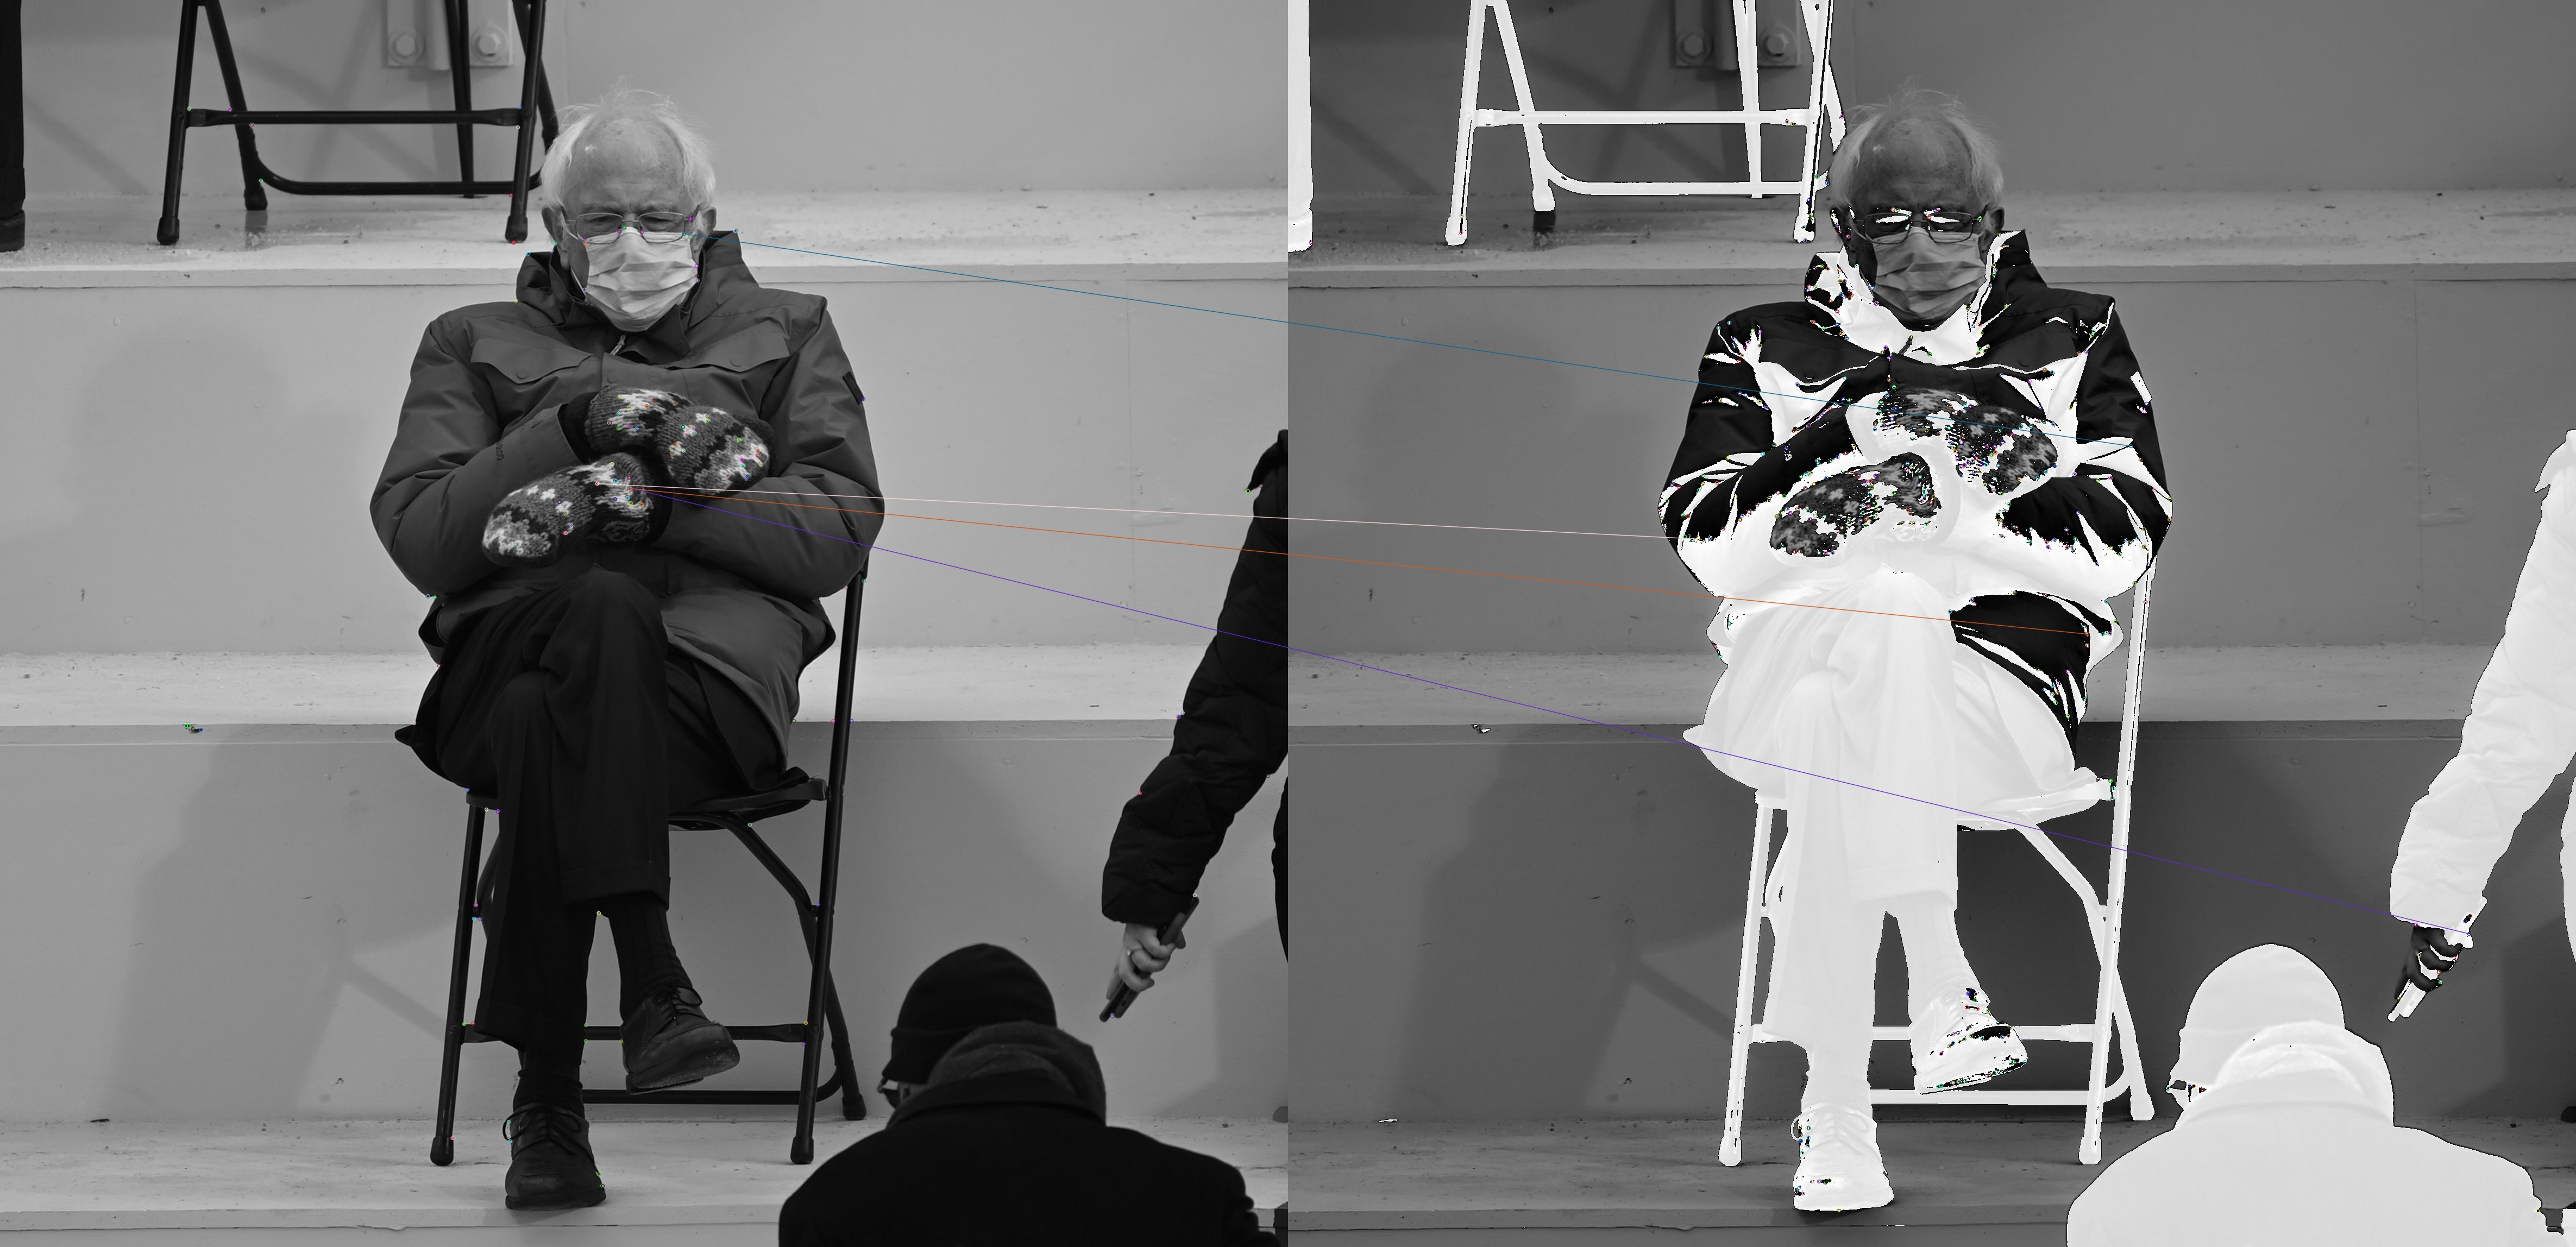
\includegraphics[width=\textwidth]{darkerBernie.jpg_match}
	\caption{Darker image}
\end{figure}

In both cases, the changes in intensities confuse the matcher greatly.

\clearpage
\subsection*{Conclusions}

Our implementation performs poorly when faced with variations. The sigma for Gaussian blurring affects how sharp the features are placed. The SSD threshold can create a lot of wrong matches even with the ratio threshold set high, especially in the case where the benchmark is at a different scale. It has been empirically found that most images do not produce low ratios between the first and second match, even for correct matches. Another way to choose the threshold for picking the keypoints algorithmically would have been to pick the top 30\% and select the lowest value as the threshold value, quantitatively choosing the threshold. Instead, we opted to use an empirical method. We believe finding good parameters to make the model perform well is a very time-consuming task for the level of experience that we possess in this moment, so we conclude by being satisfied that we have reached this far. This is an excellent point from which to start further studies in Computer Vision.

\clearpage
\section*{Appendix}

\begin{figure}[hb]
	\centering
	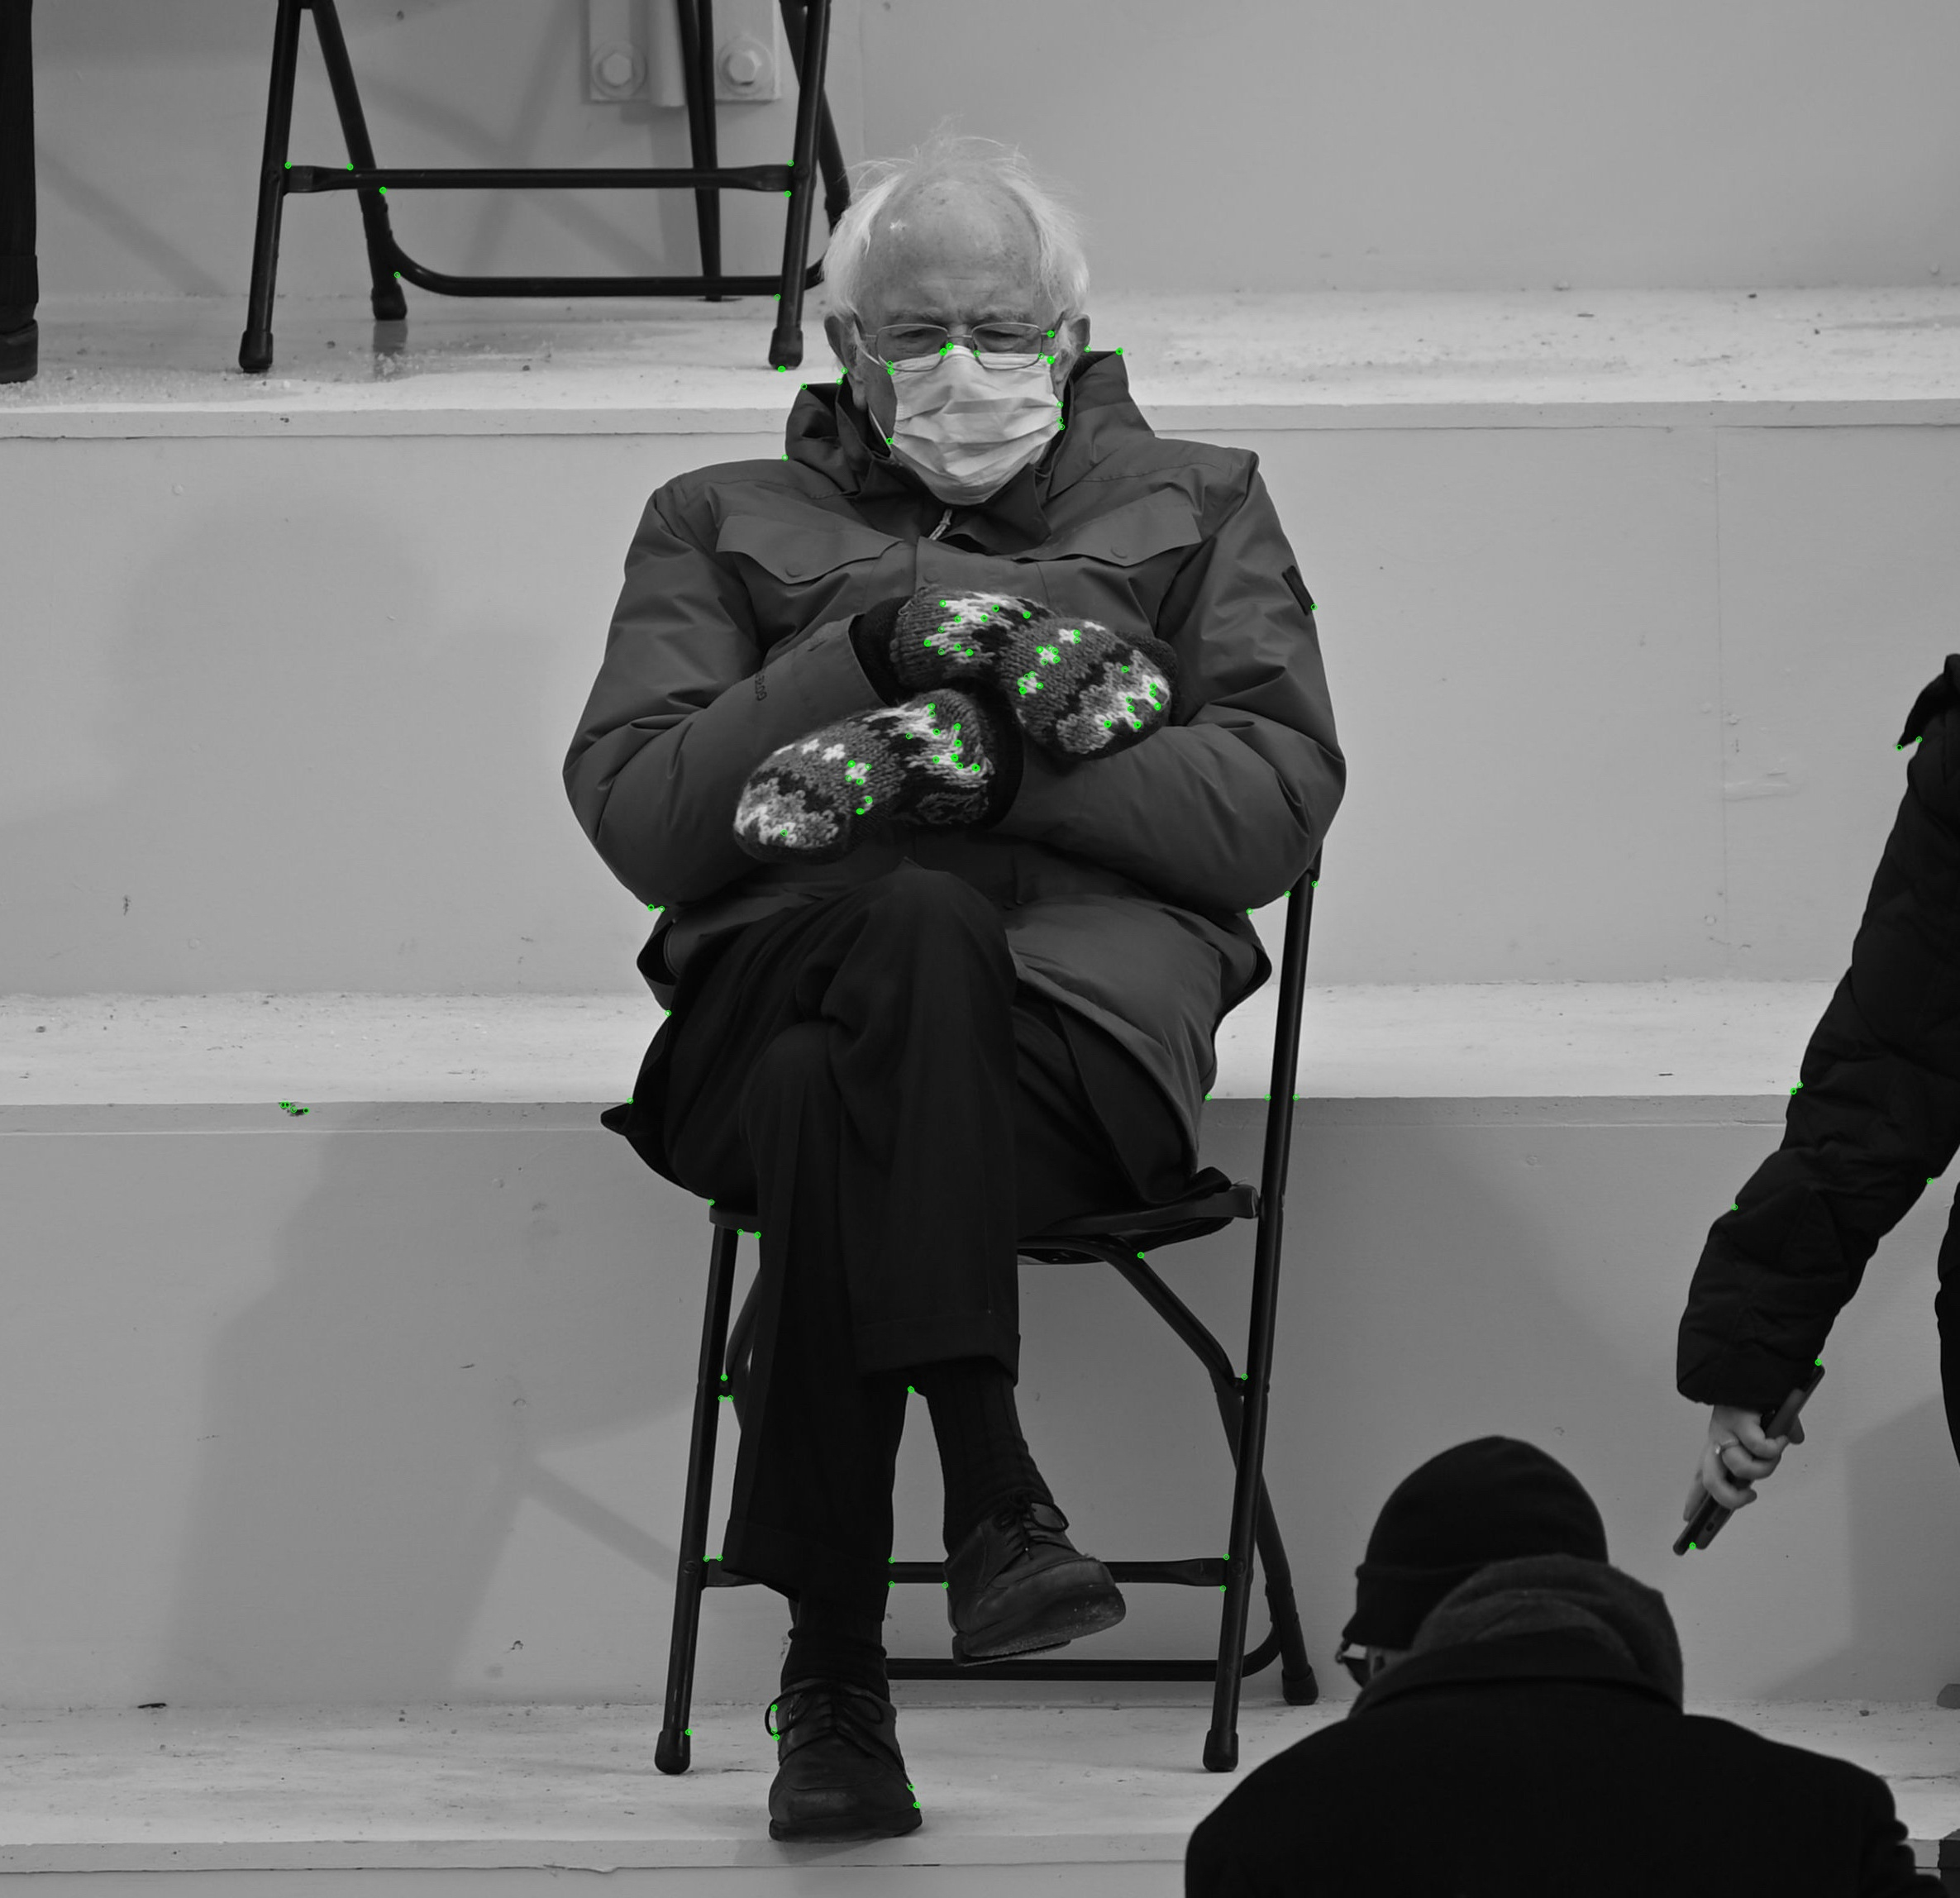
\includegraphics[width=\textwidth]{orig_keypoints}
	\caption{Reference image}
\end{figure}

\begin{figure}[hb]
	\centering
	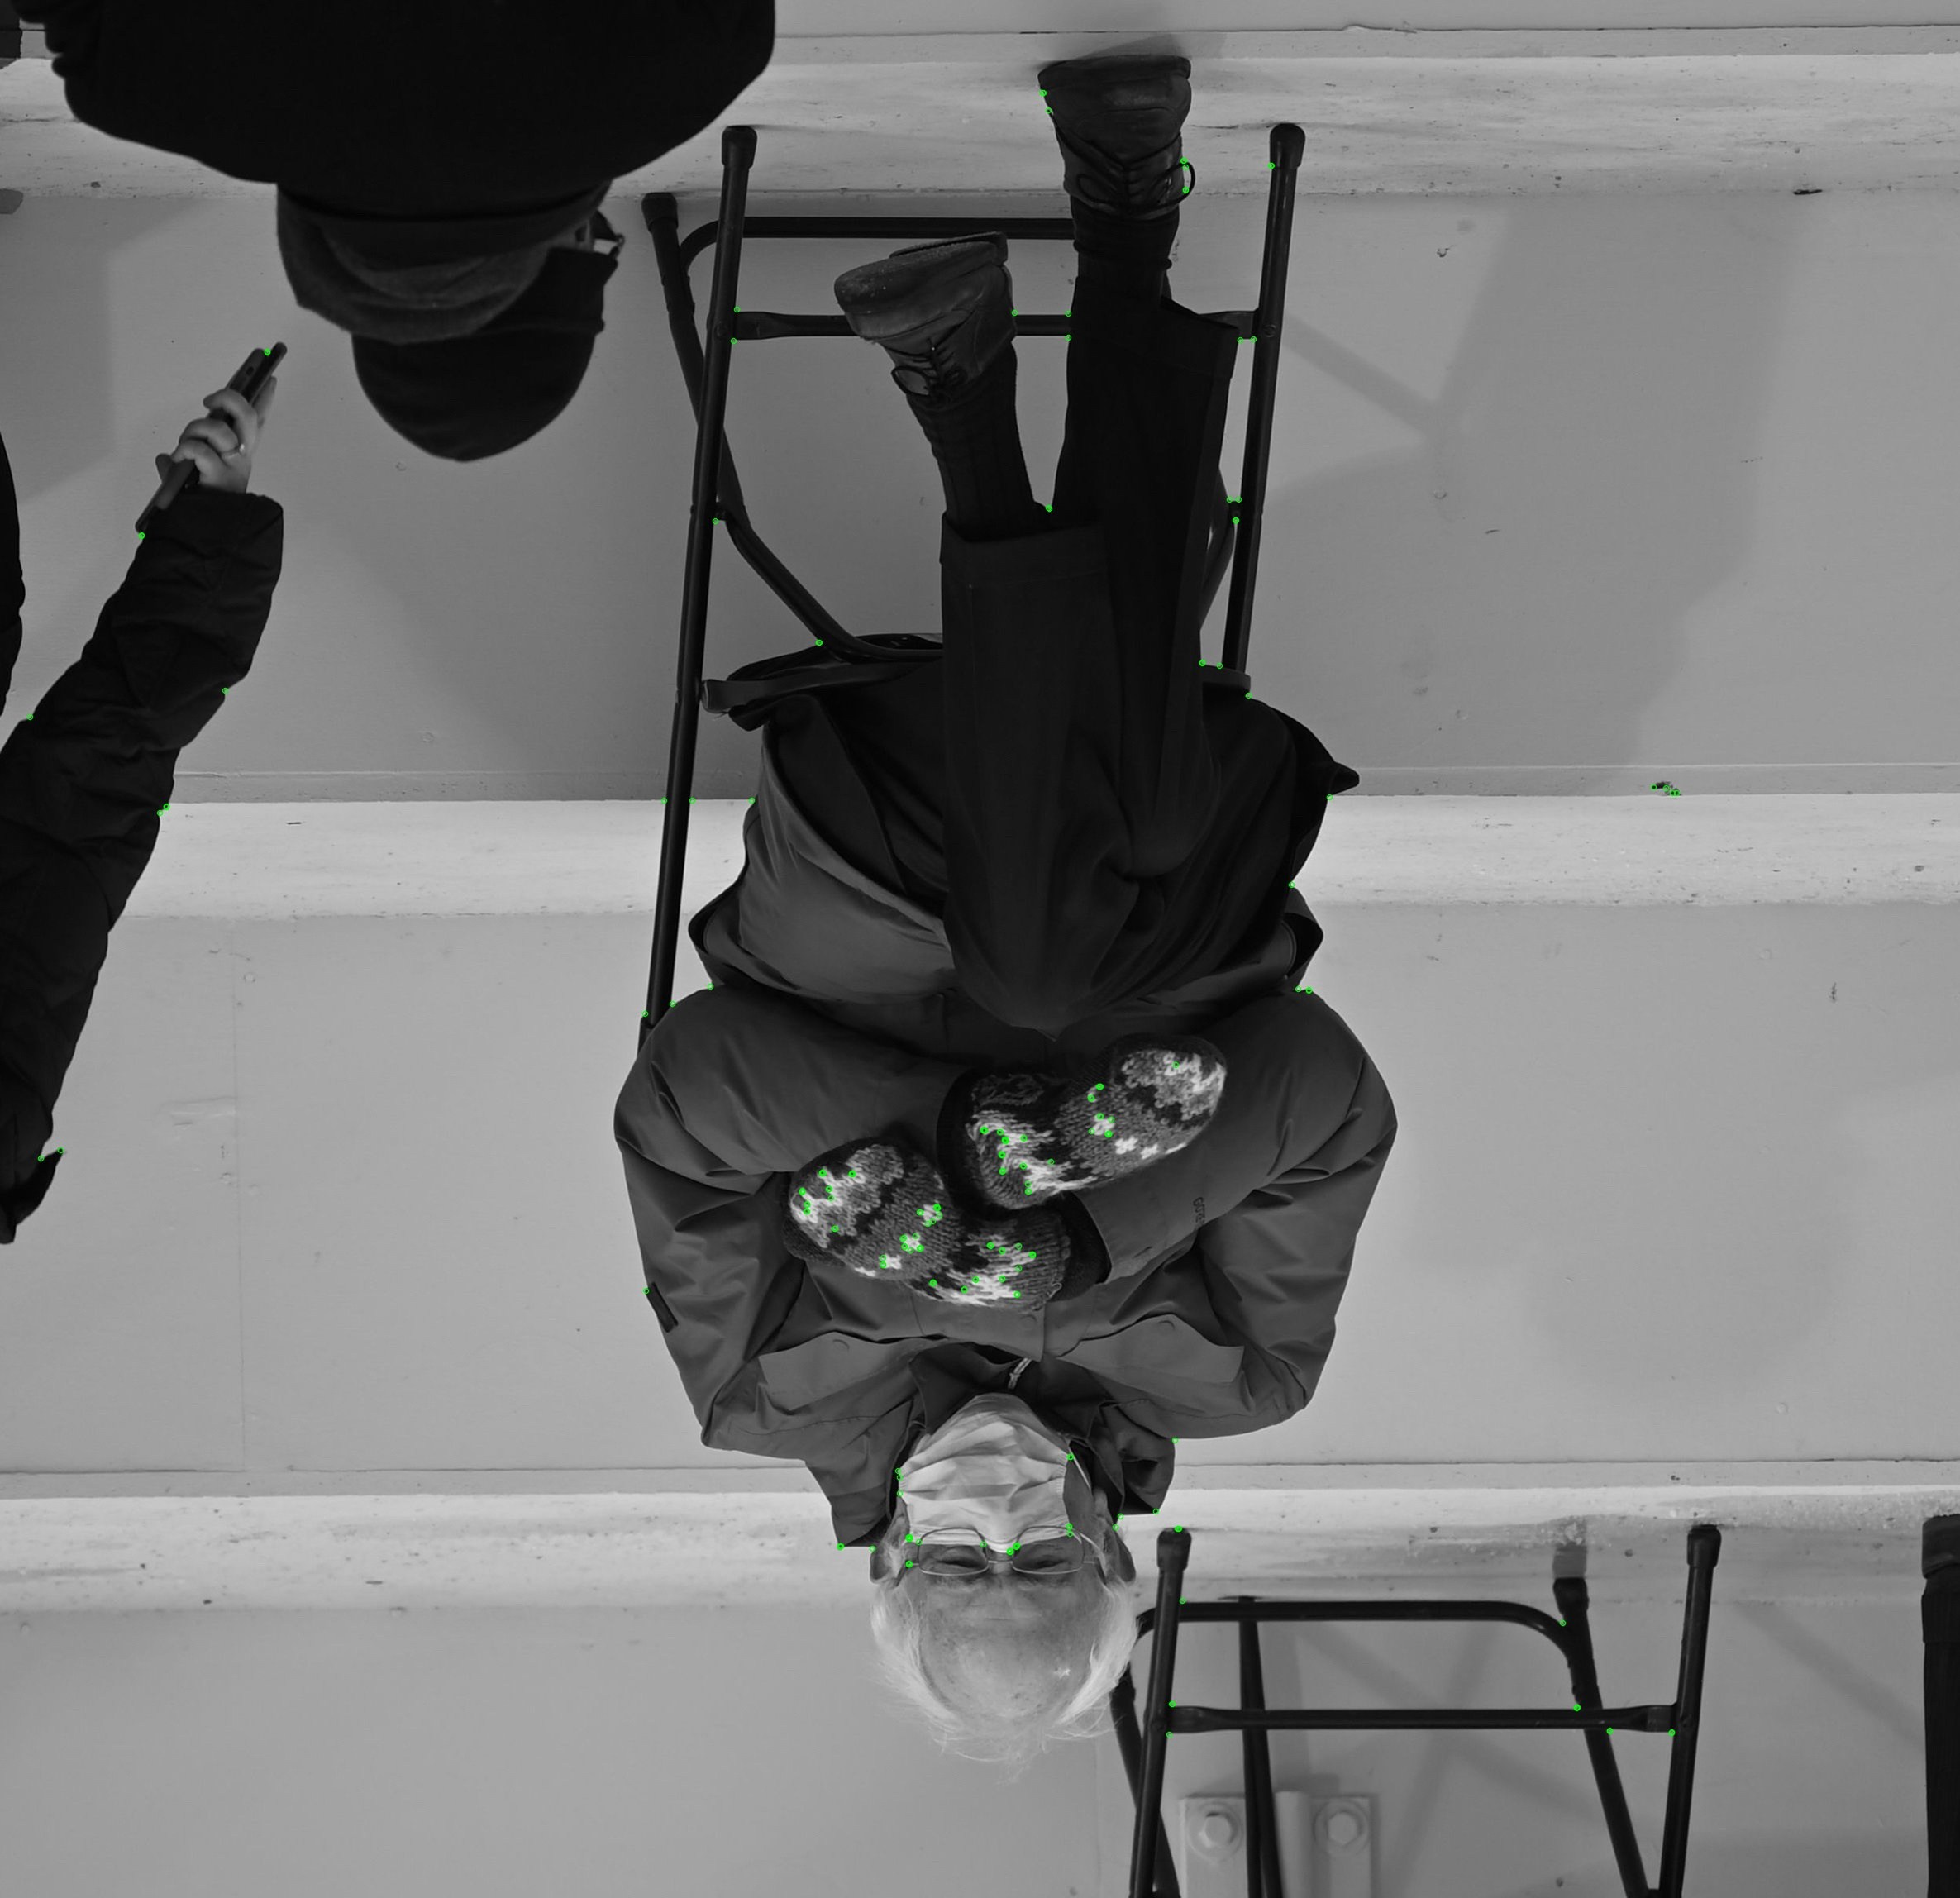
\includegraphics[width=\textwidth]{bernie180.jpg_keypoints}
	\caption{Rotated image}
\end{figure}

\begin{figure}[hb]
	\centering
	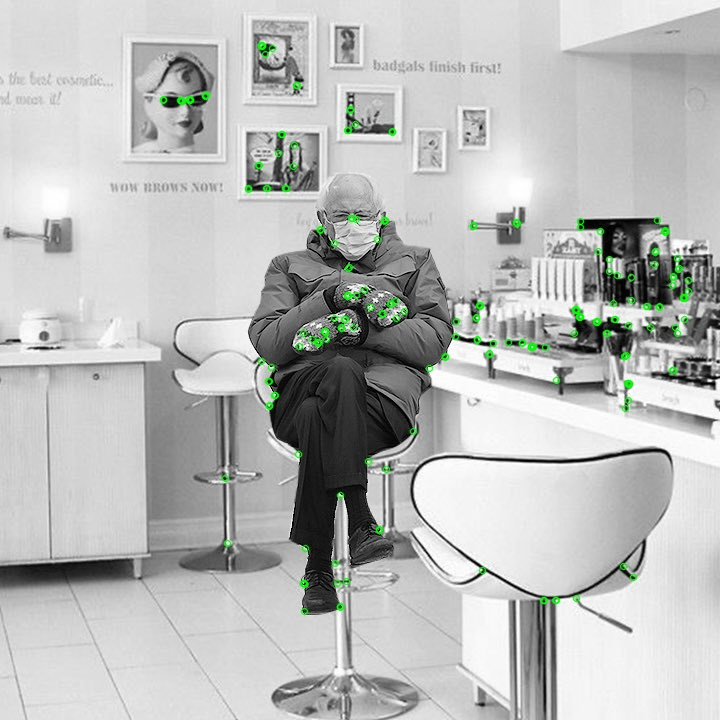
\includegraphics[width=\textwidth]{bernieBenefitBeautySalon.jpeg_keypoints}
	\caption{Scaled image}
\end{figure}
\begin{figure}[hb]
	\centering
	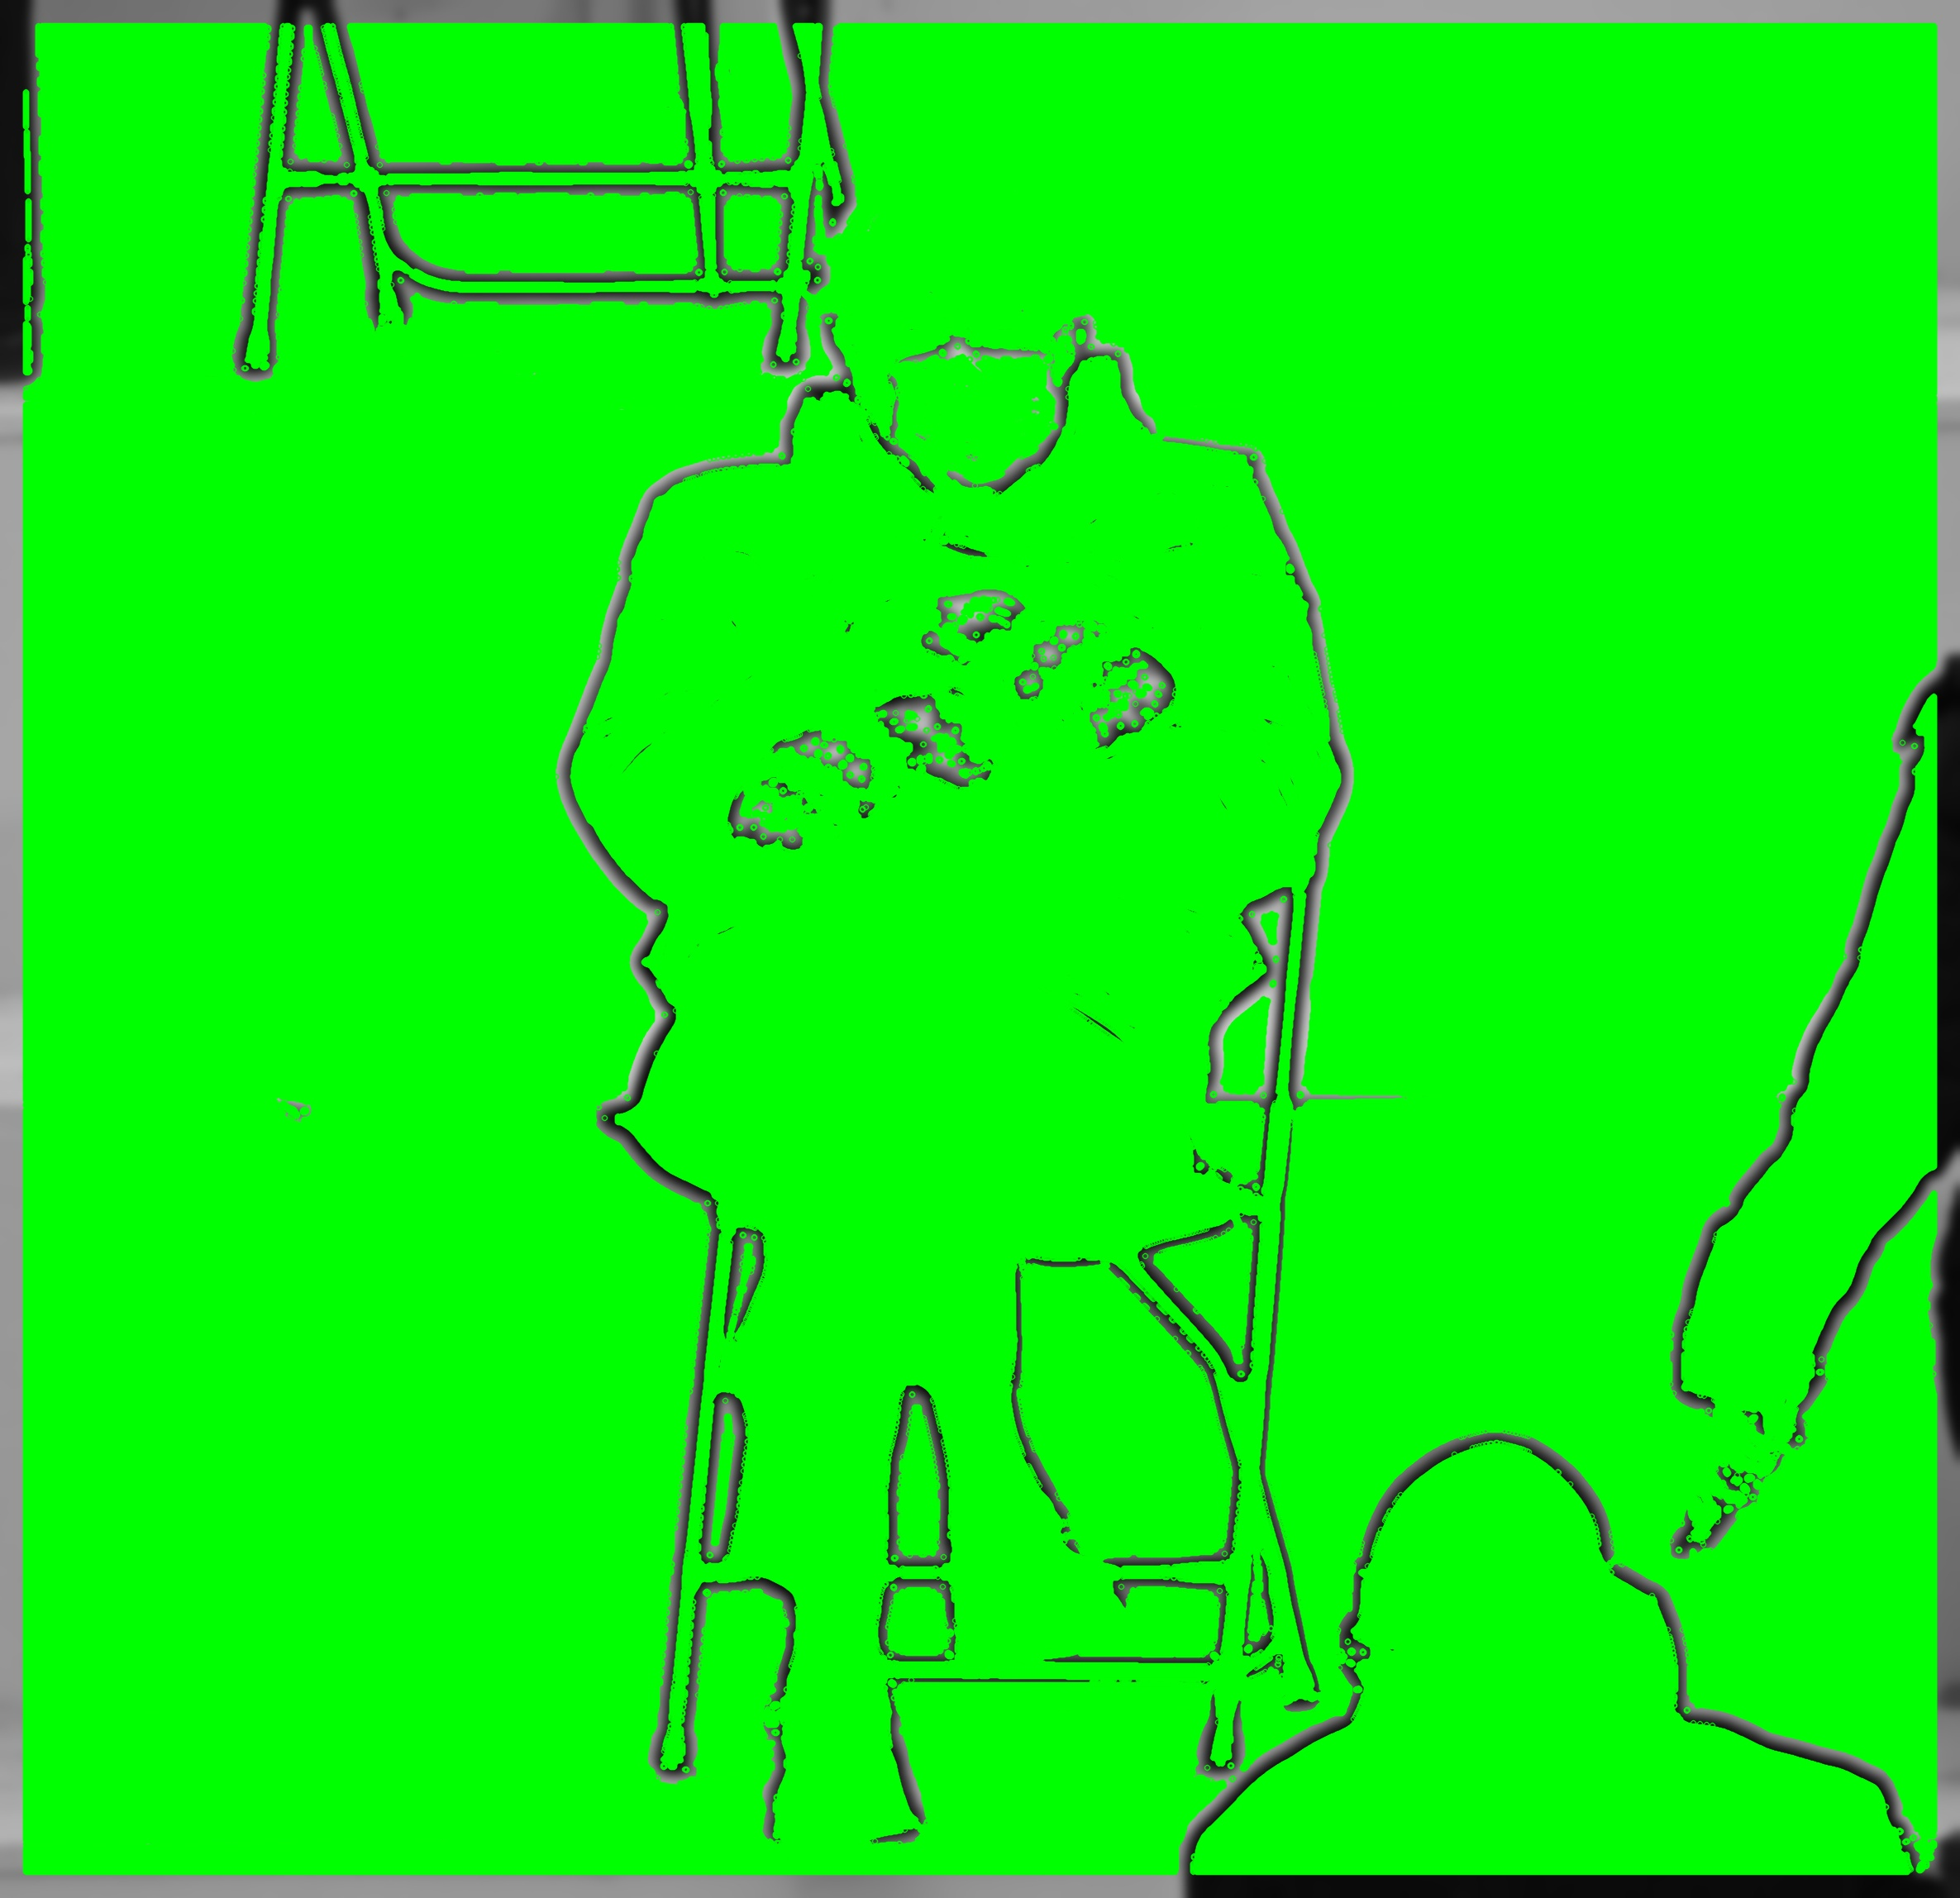
\includegraphics[width=\textwidth]{bernieMoreblurred.jpg_keypoints}
	\caption{Blurred image image}
\end{figure}
\begin{figure}[hb]
	\centering
	\includegraphics[width=\textwidth]{bernieNoisy2.png_keypoints}
	\caption{Noisy image}
\end{figure}
\begin{figure}[hb]
	\centering
	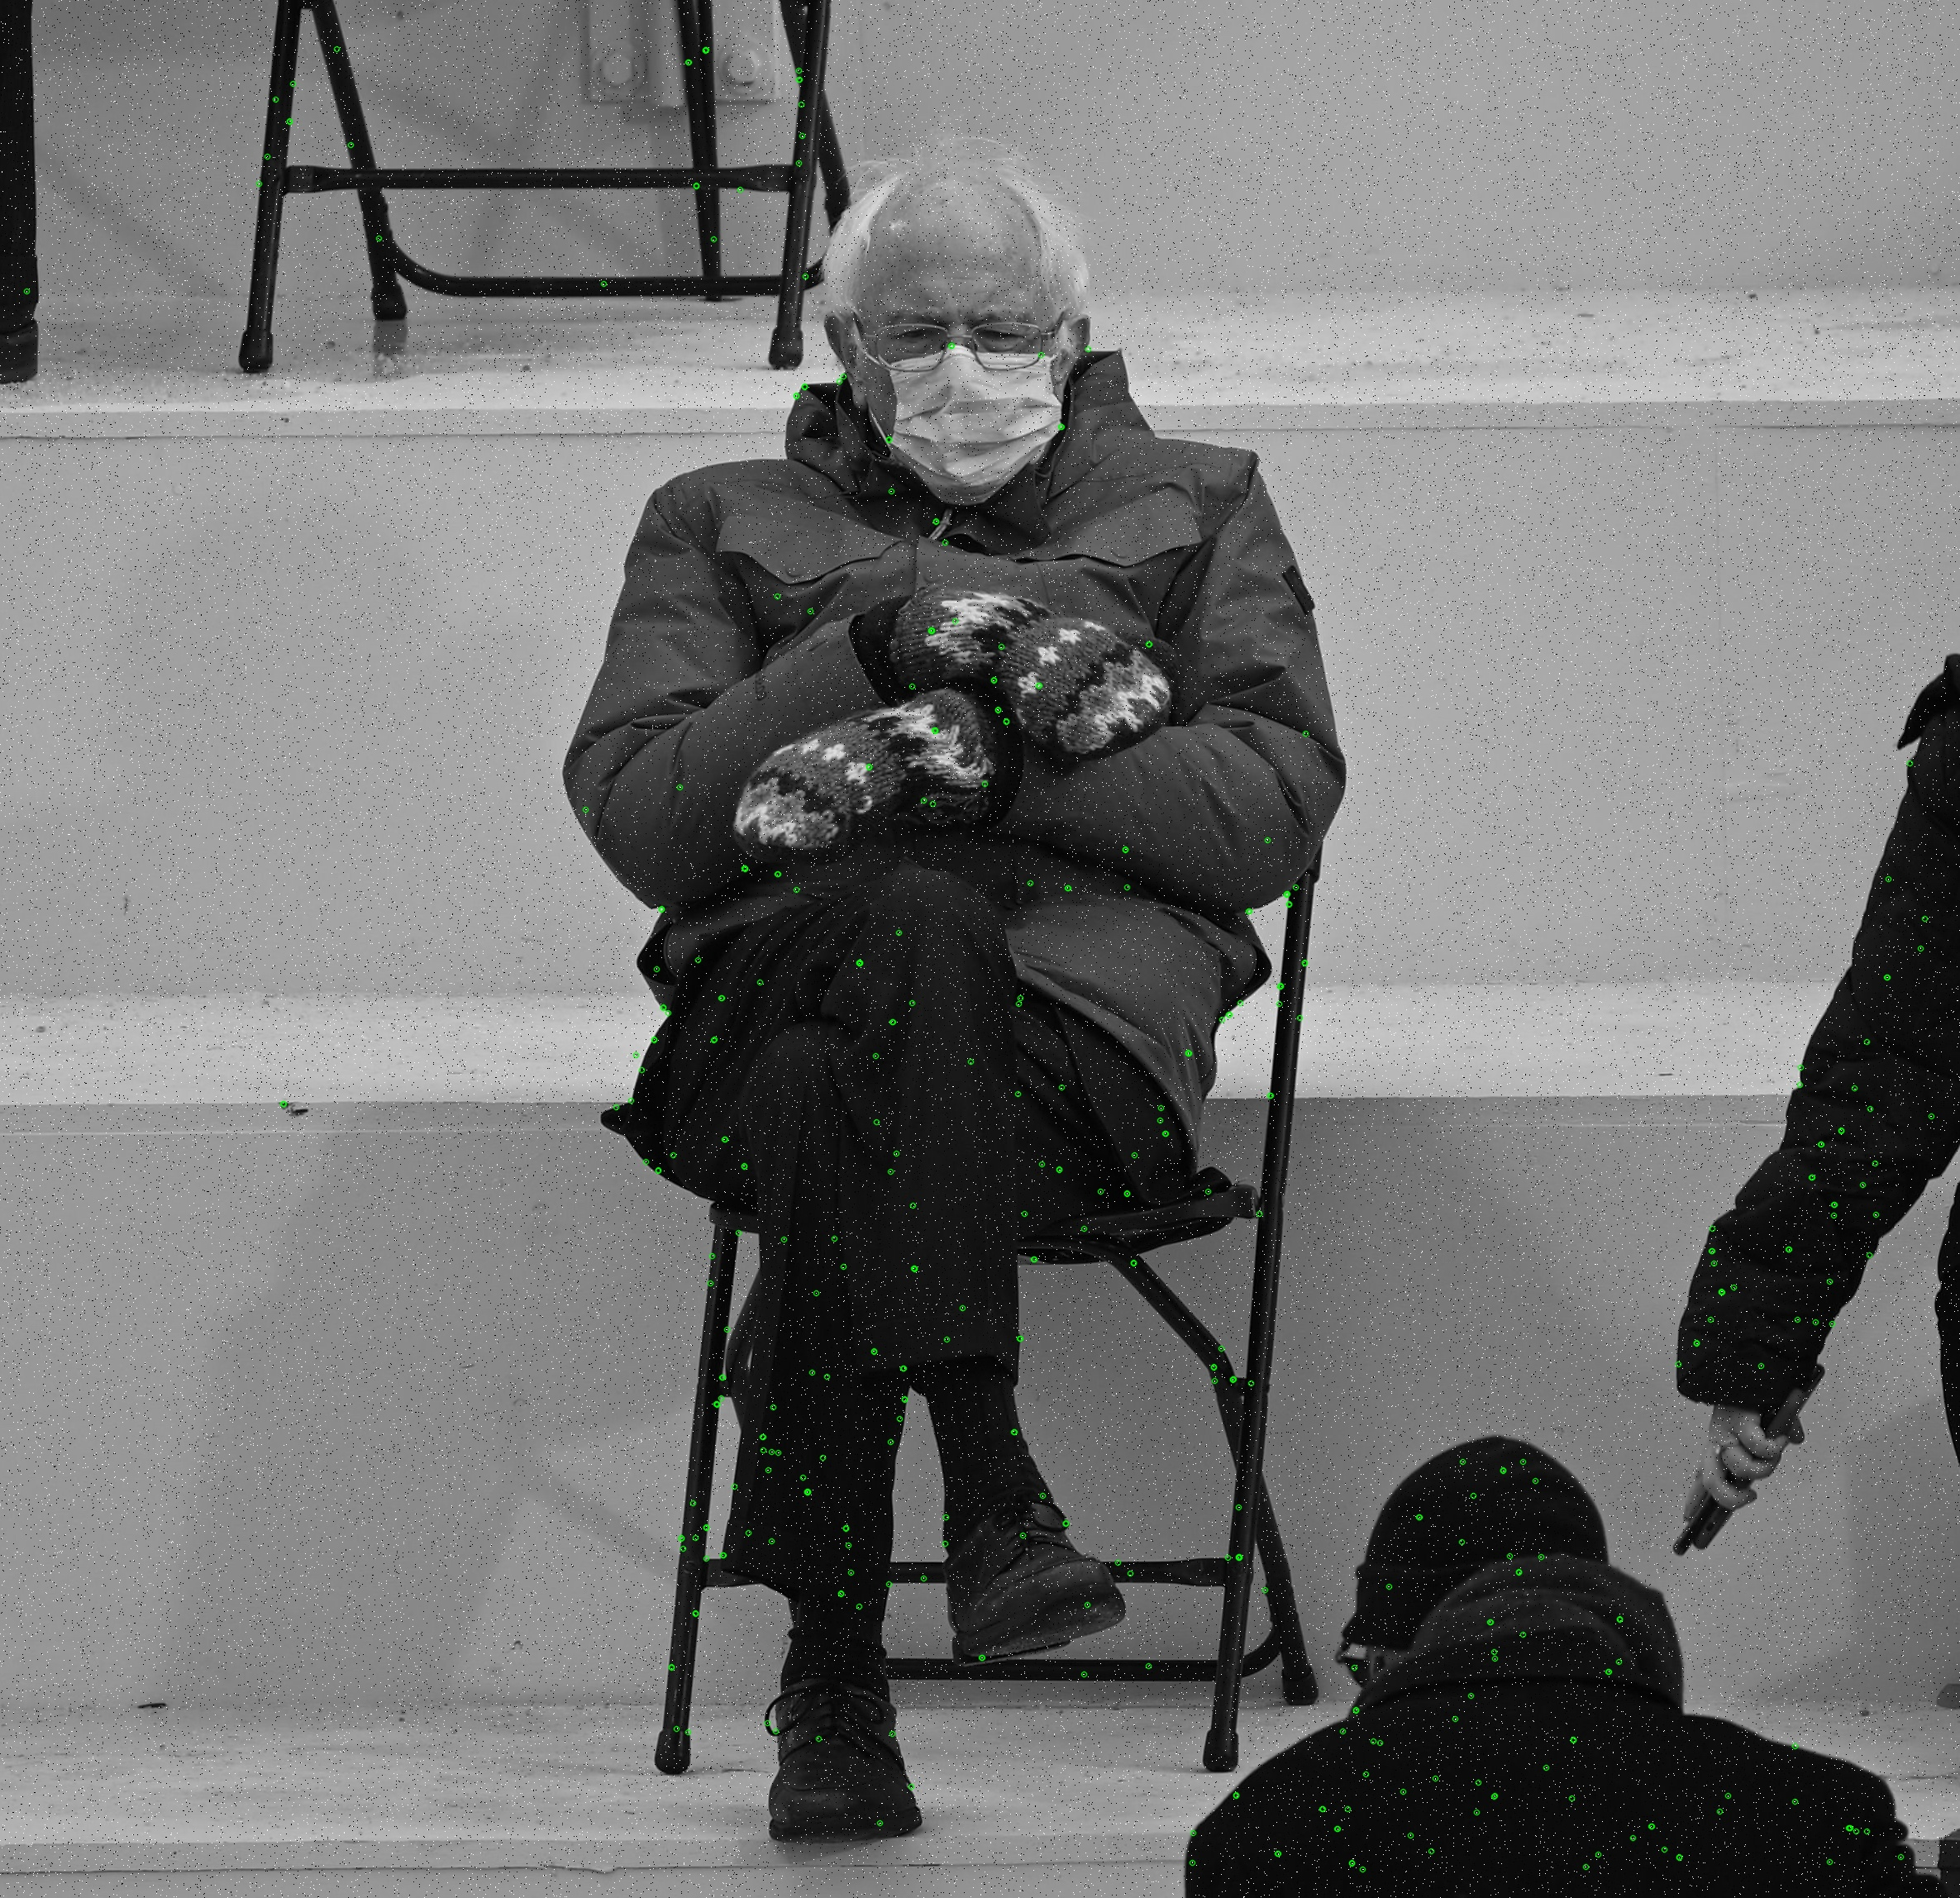
\includegraphics[width=\textwidth]{berniePixelated2.png_keypoints}
	\caption{Pixelated image}
\end{figure}
\begin{figure}[hb]
	\centering
	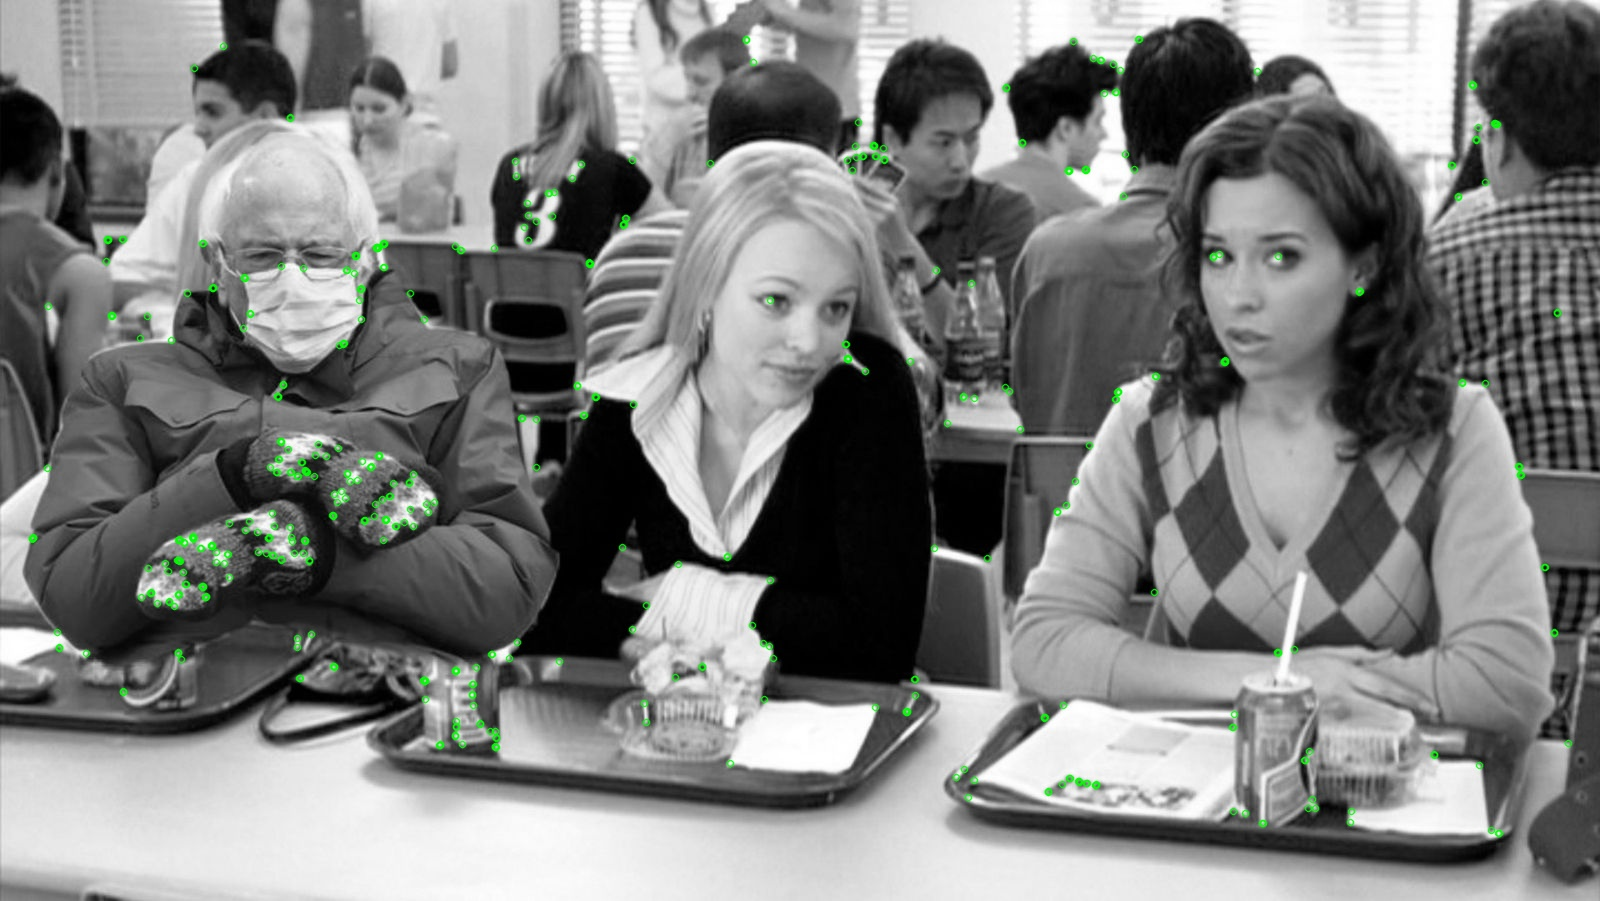
\includegraphics[width=\textwidth]{bernieShoolLunch.jpeg_keypoints}
	\caption{Similar characters and scaled image}
\end{figure}
\begin{figure}[hb]
	\centering
	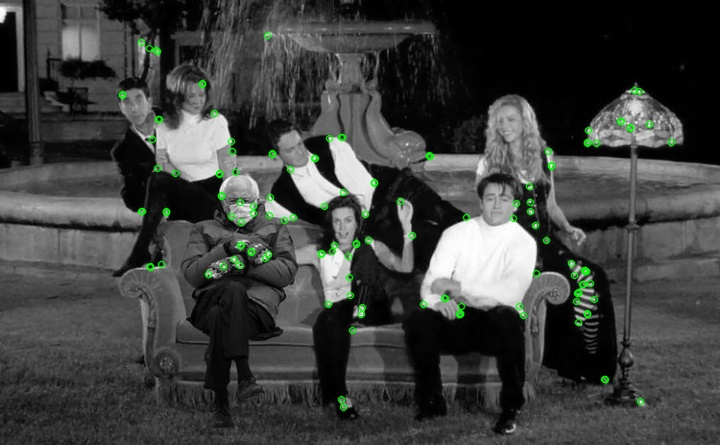
\includegraphics[width=\textwidth]{BernieFriends.png_keypoints}
	\caption{Many characters and scaled image}
\end{figure}
\begin{figure}[hb]
	\centering
	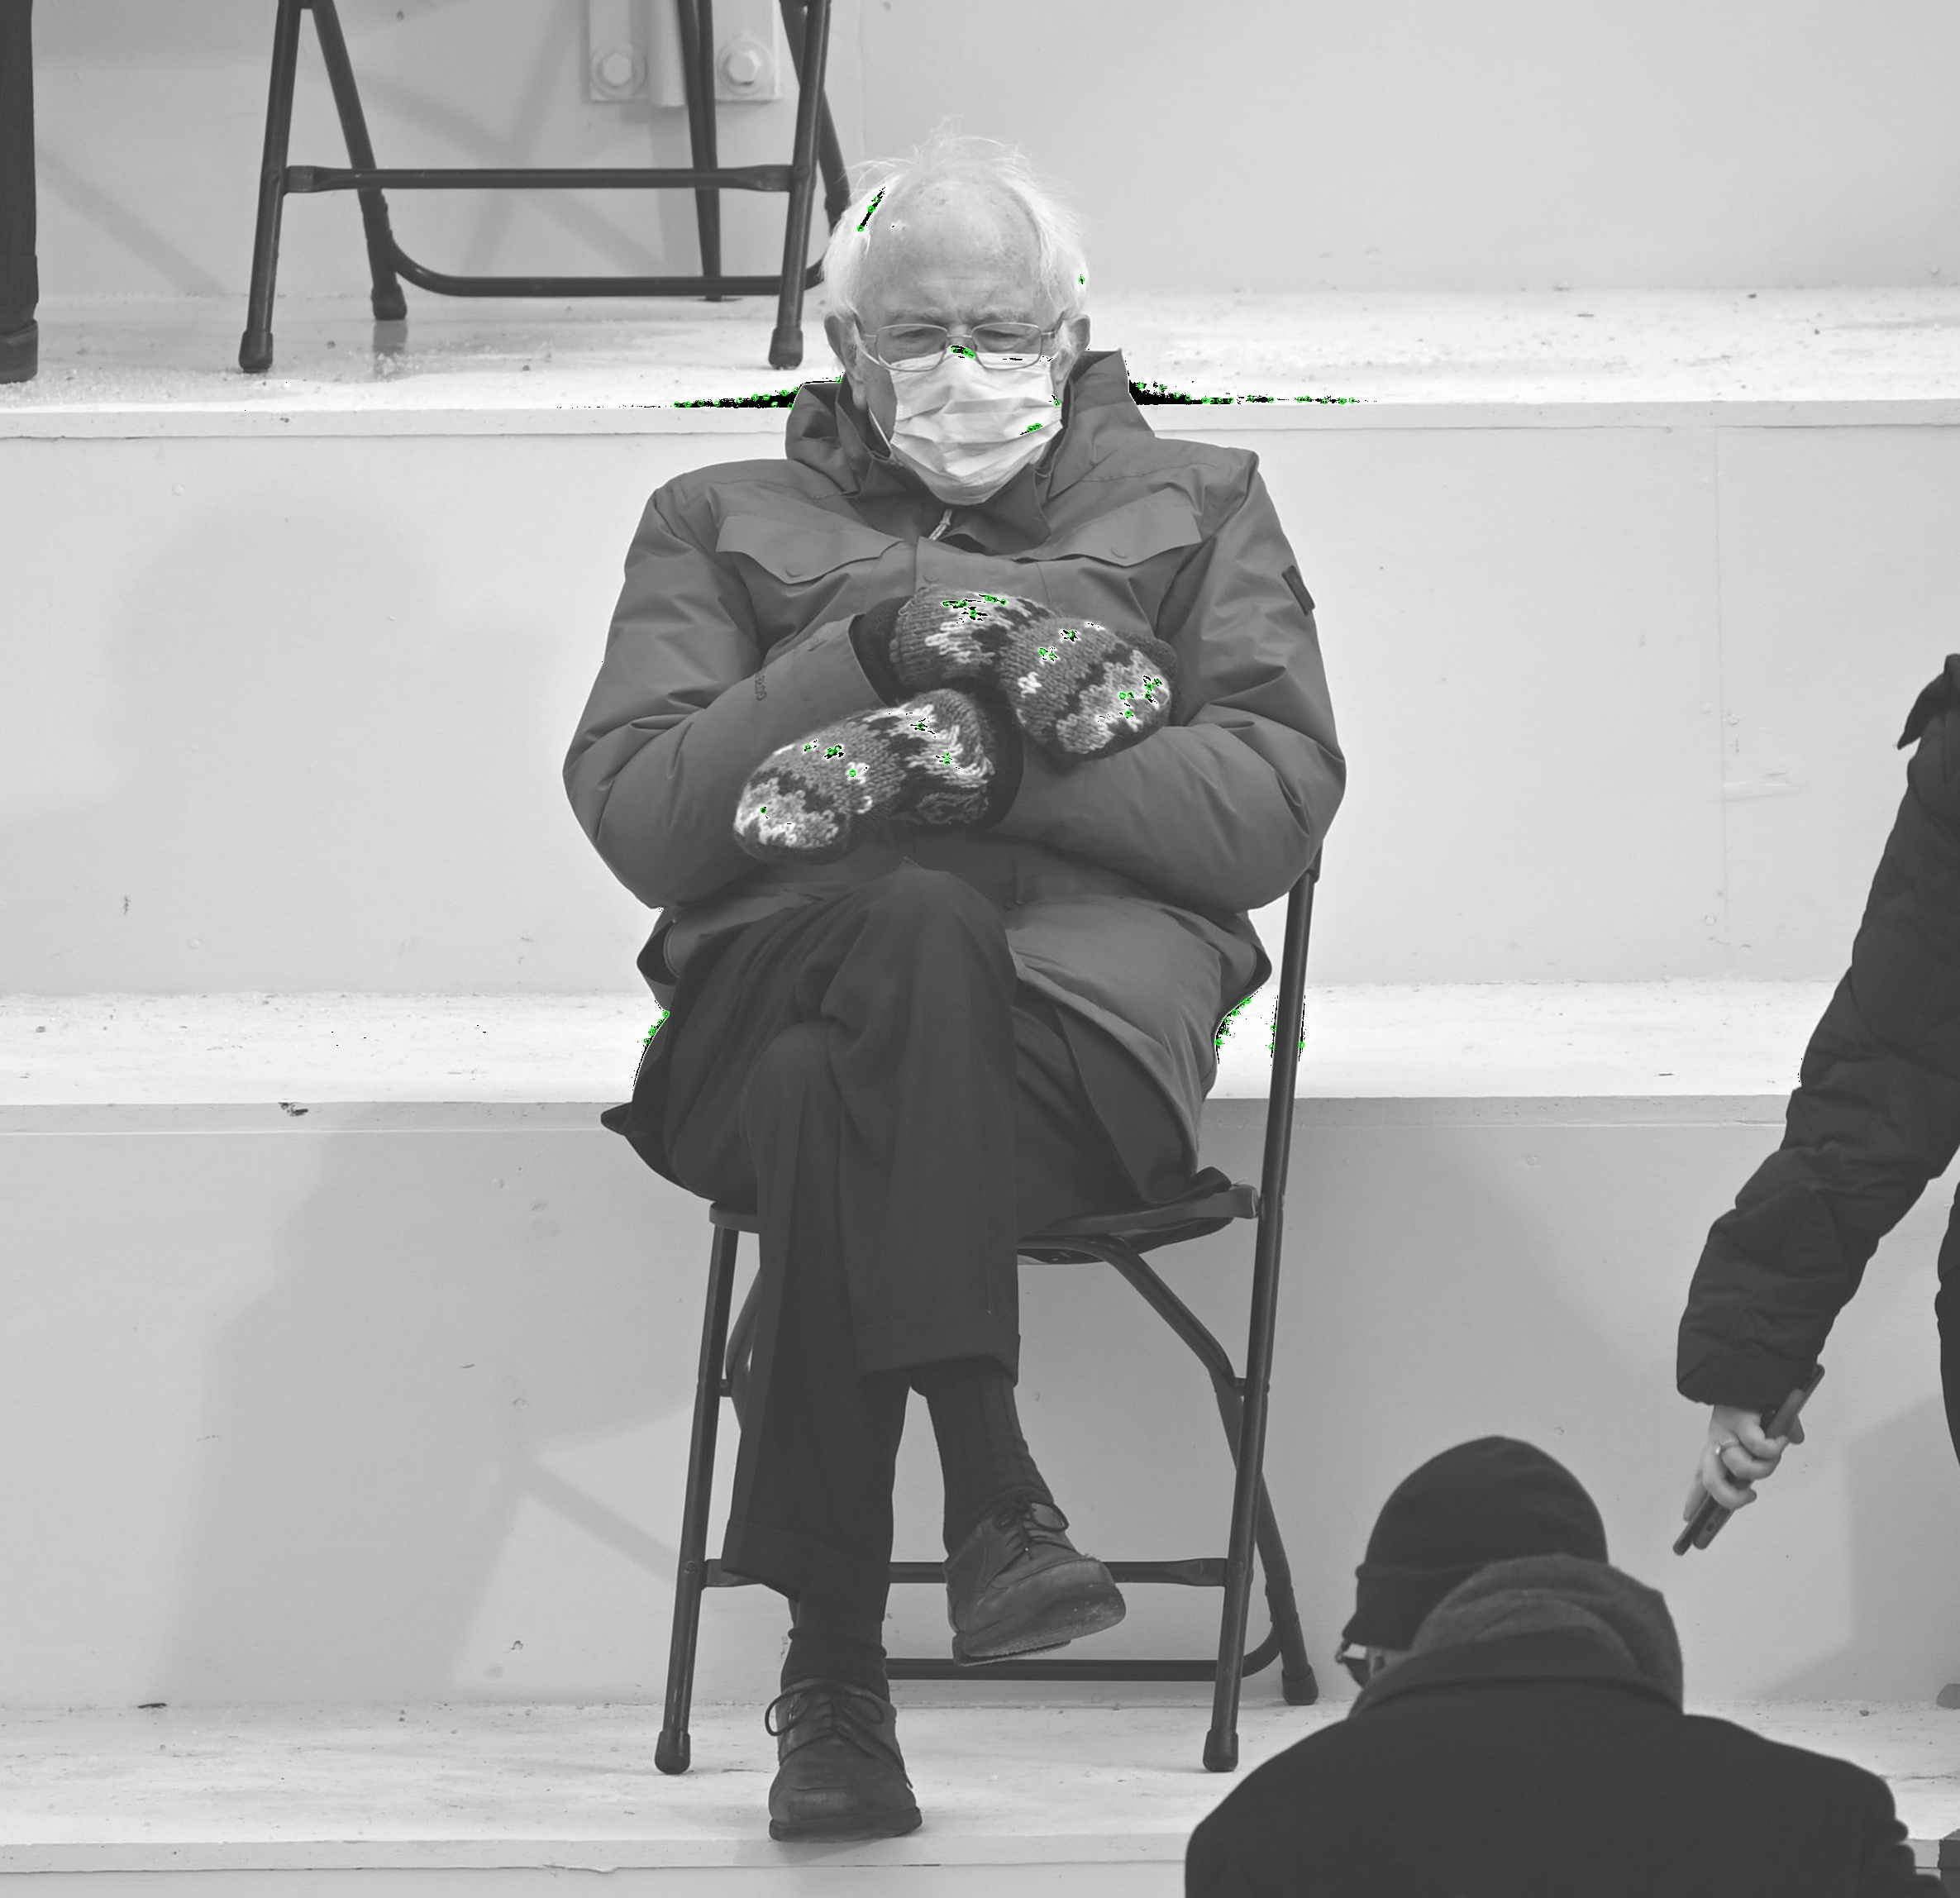
\includegraphics[width=\textwidth]{brighterBernie.jpg_keypoints}
	\caption{Brighter image}
\end{figure}
\begin{figure}[hb]
	\centering
	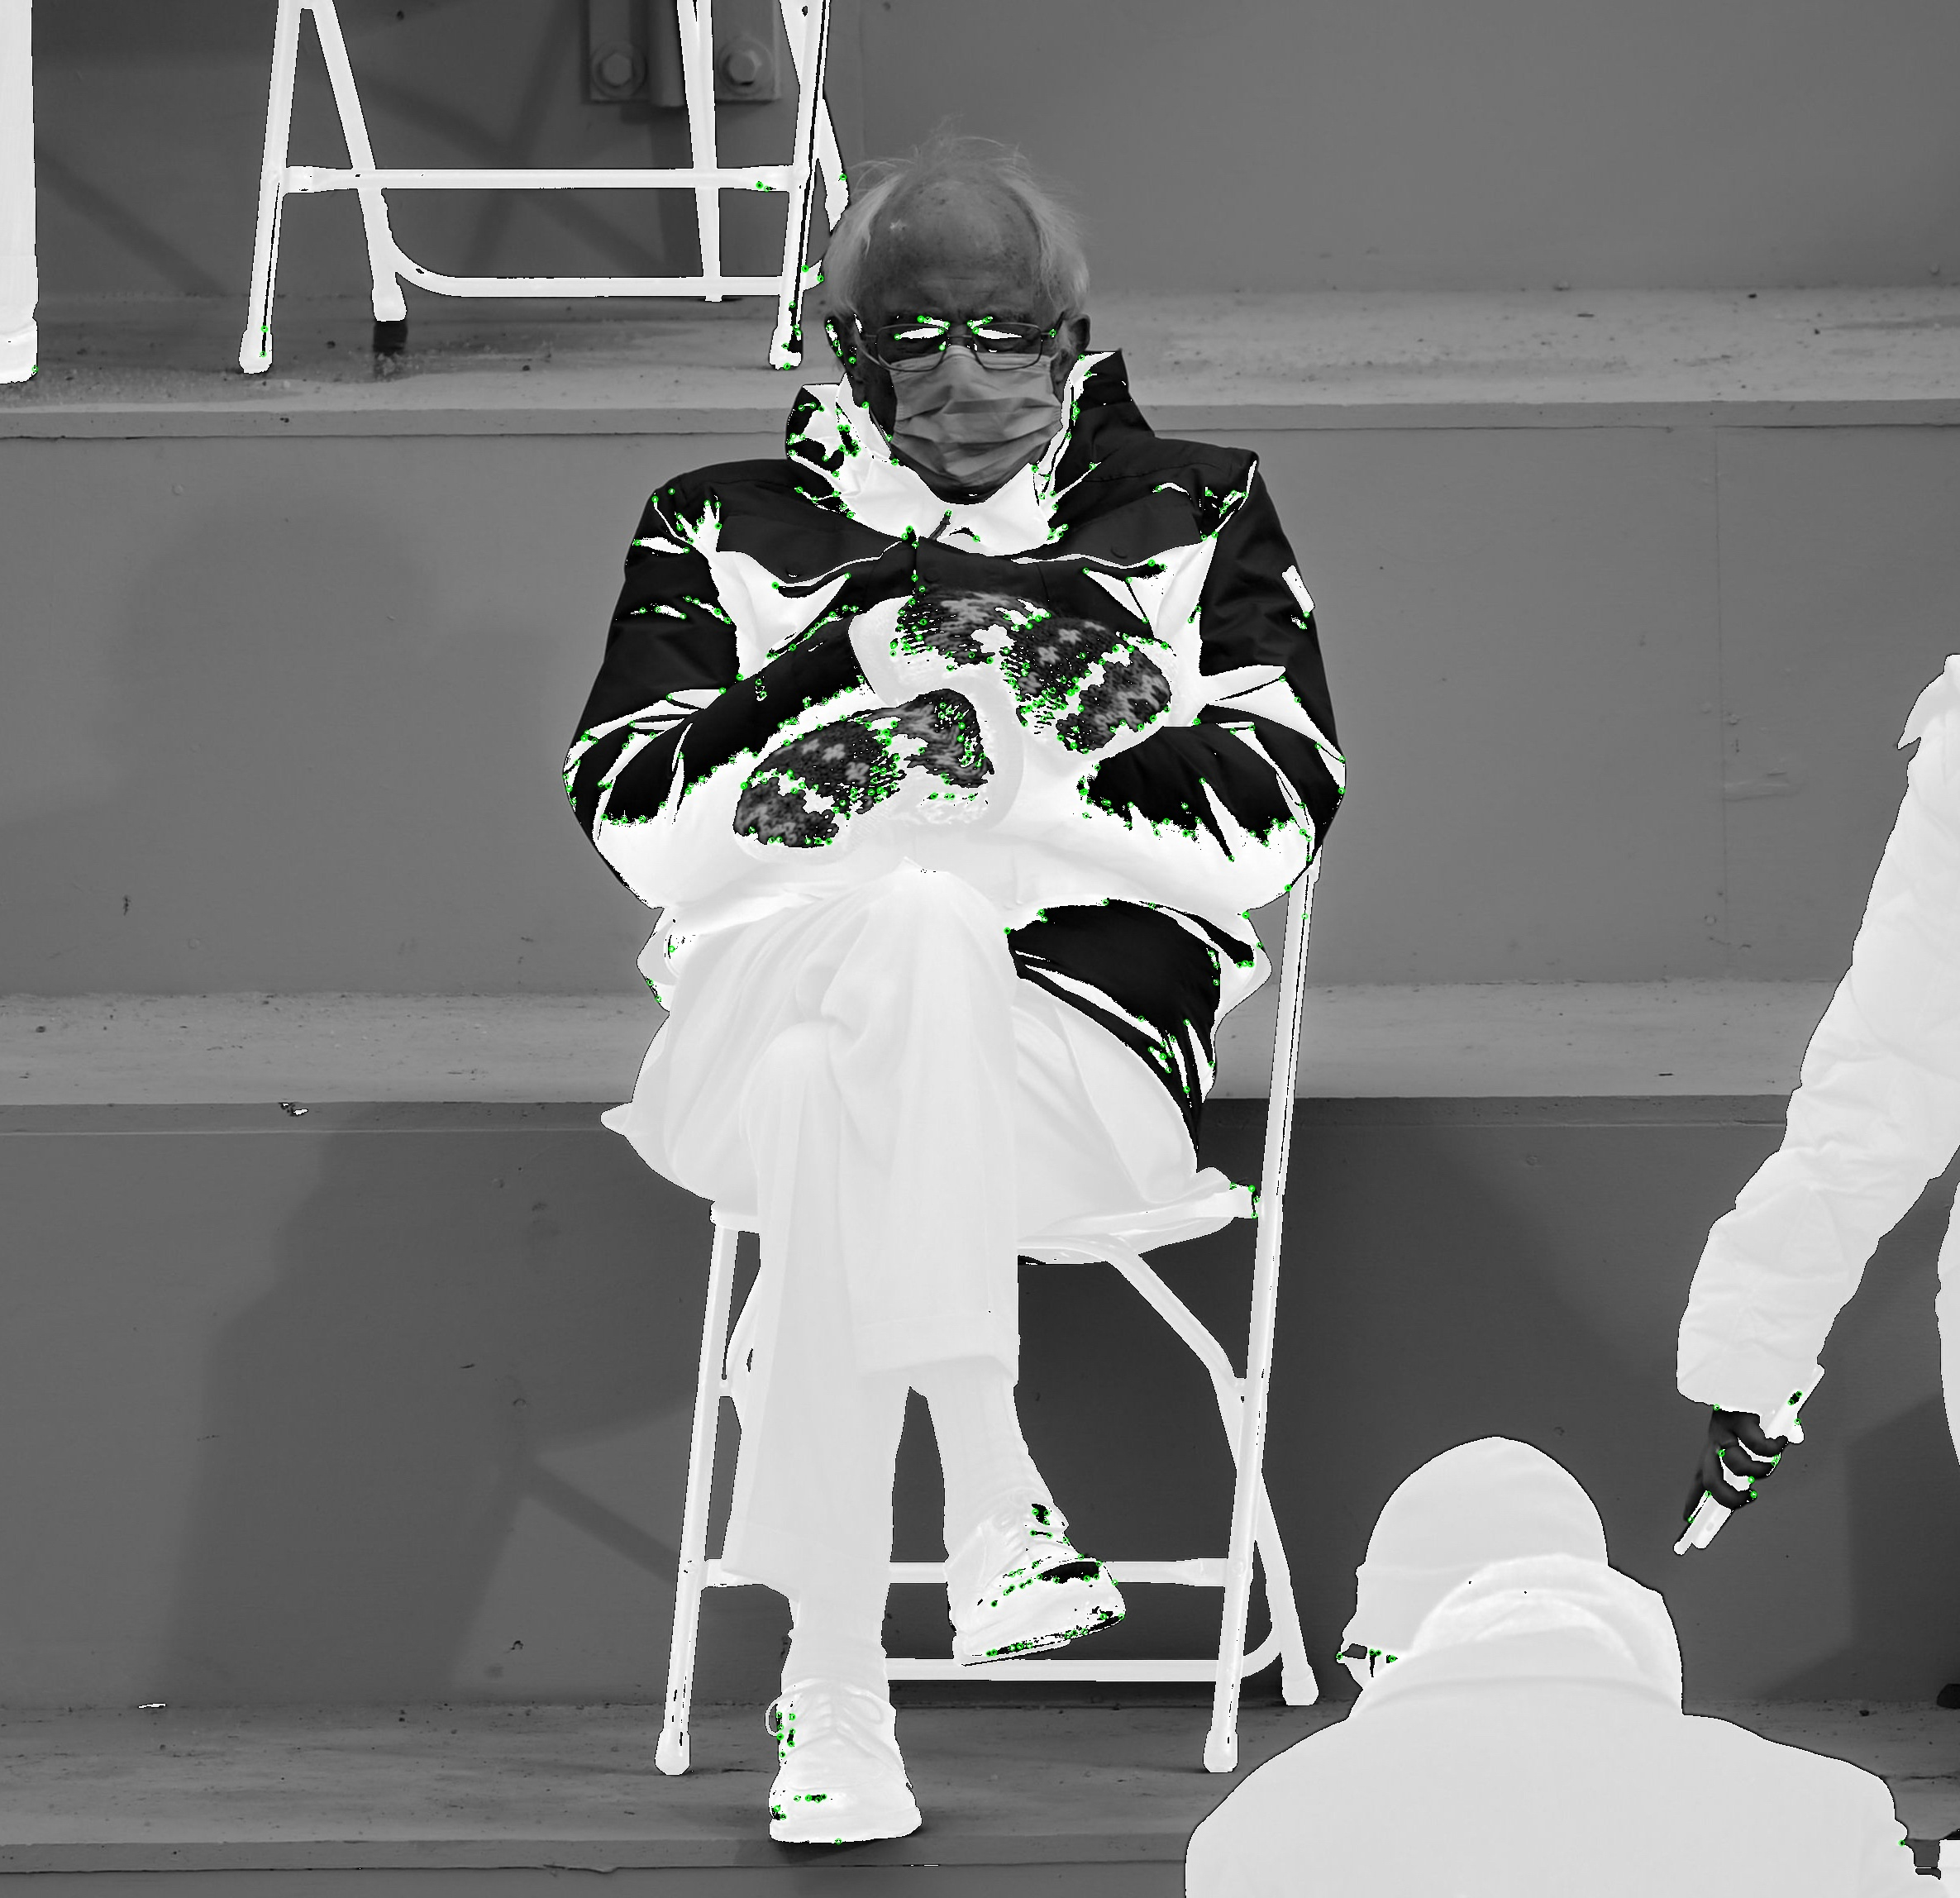
\includegraphics[width=\textwidth]{darkerBernie.jpg_keypoints}
	\caption{Darker image}
\end{figure}

\end{document}